\chapter{Experiments}
\label{c:experiments}

We use 25 benchmark problems from the CEC 2005 Special Session on Real-Parameter Optimization to test the performance of our new techniques.
The CEC 2005 benchmark problems are composed of both standard test problems e.g. Sphere, Schwefel's, Rosenbrock's, Rastrigin's, etc.,
and some hybrid problems.
We tested the CMA-ES, PSO, and ACO$_R$ algorithms with and without our new techniques.
The results show that our technique reduces the average error of CMA-ES and ACO$_R$ on some multimodal problems.  



\section{CEC2005 25 benchmark problems}

The CEC 2005 Special Session on Real-Paramter Optimization~\cite{Suganthan:2005:benchmark} aims to evaluate different algorithms in a more systematic manner by specifying a common termination criterion, size of problems, linkages/rotation, etc.
It consists of 25 minimization problems with $2, 10, 30, 50$ dimensions.
The evaulation requires 25 runs, each with maximum evaluations $10000 * D$. 
Initialization is required to be uniform random within the search space, except for problems 7 and 25, for which initialization ranges are specified.
Similarly, the global optimum exists within the given bounds, except for problem 7 and 25.
The algorithm is terminated one it reaches the maximum evaluations or if the minimum error in the function value is less than $10^{-8}$.
Here we only tested on the 2-dimensional problems, 
since our technique consumes too much time on higher dimensions, 
making optimization impractical.  
Further speedup and studies to expend the technique on higher dimension are needed.
We show the average and median error plots for all 25 problems in the following section.
The tables, following the requested format in~\cite{Suganthan:2005:benchmark}, are also given the the following section.  

\section{Experiment Settings}

In this section, we breifly describe the parameters setting for CMA-ES, SPSO and ACOR.

We use the \textit{Covariance Matrix Adaptation Evolution Strategy for non-linear numerical optimization in Python} package~\footnote{https://pypi.python.org/pypi/cma} provided by Hensen, the author of CMA-ES.
Although the default population for CMA-ES in $D$-dimension is set to be $4 + \lfloor3\log(D)\rfloor$, meaning default population size is 6 in 2D,
we found out that we a larger population for the MDL to not merge every particles into one cluster.
Therefore, we set the population size as 30 for CMA-ES.
The initial mean is set to be the center between max bounds and min bounds $(max_d + min_d)/2$ in every dimension.
The initial sigma is set to be one sixth of the maximum length between max bounds and min bounds in each dimension $\max_{d}(max_d - min_d)/6$.
It is suggested to let the global optimum be within three sigma~\cite{Hansen:2006:CMA_ES_review}.

As for th SPSO 2011, there are currently no official Python implementation, 
so we created our own Python implementation according to the tutorials~\cite{Clerc:2012:SPSO2011}~\cite{Clerc:2007:randomTopology},
and the official C++ code~\footnote{https://www.particleswarm.info/standard\_pso\_2011\_c.zip} provided Clerc.
The population size is set to be 40 as suggested in~\cite{Clerc:2012:SPSO2011}.
The parameters $c = \frac{1}{2} + \ln(2) \simeq 1.193$ and $w = \frac{1}{2\ln(2)} \simeq 0.721$ are also set as default.
We implement the random topology with $K = 3$,
and update the topology at the beginning and in every iteration when the best fitness does not improve.
Also, we use the ``bounce back'' boundary condition suggested in~\cite{Clerc:2012:SPSO2011}, which is also described in Chapter~\ref{chapter:algos}.


For ACOR, we set our parameters according to the original paper~\cite{Socha:2008:ACOR}. 
The parameters are shown in Table~\ref{table:ACOR_parameters}.

\begin{table}%[t!]
\centering
\label{table:ACOR_parameters}
\begin{tabular}{lll}
\hline
Parameter                        & Symbol   & Value          \\ \hline
No. of ants used in an iteration & $m$      & $2$            \\
Speed of convergence             & $\xi$    & $0.85$         \\
Locality of the search process   & $q$      & $10^{-4}$      \\
Archive size                     & $k$      & $50$           \\ \hline
\end{tabular}
\caption{Summary of the parameters used by $ACO_R$}
\end{table}

%Describe our bandit parameters setting, including the initial population, maximum number of arms, and (1+1)-ES step size.

\section{Experiment Results} 

%\begin{figure}
%\centering
%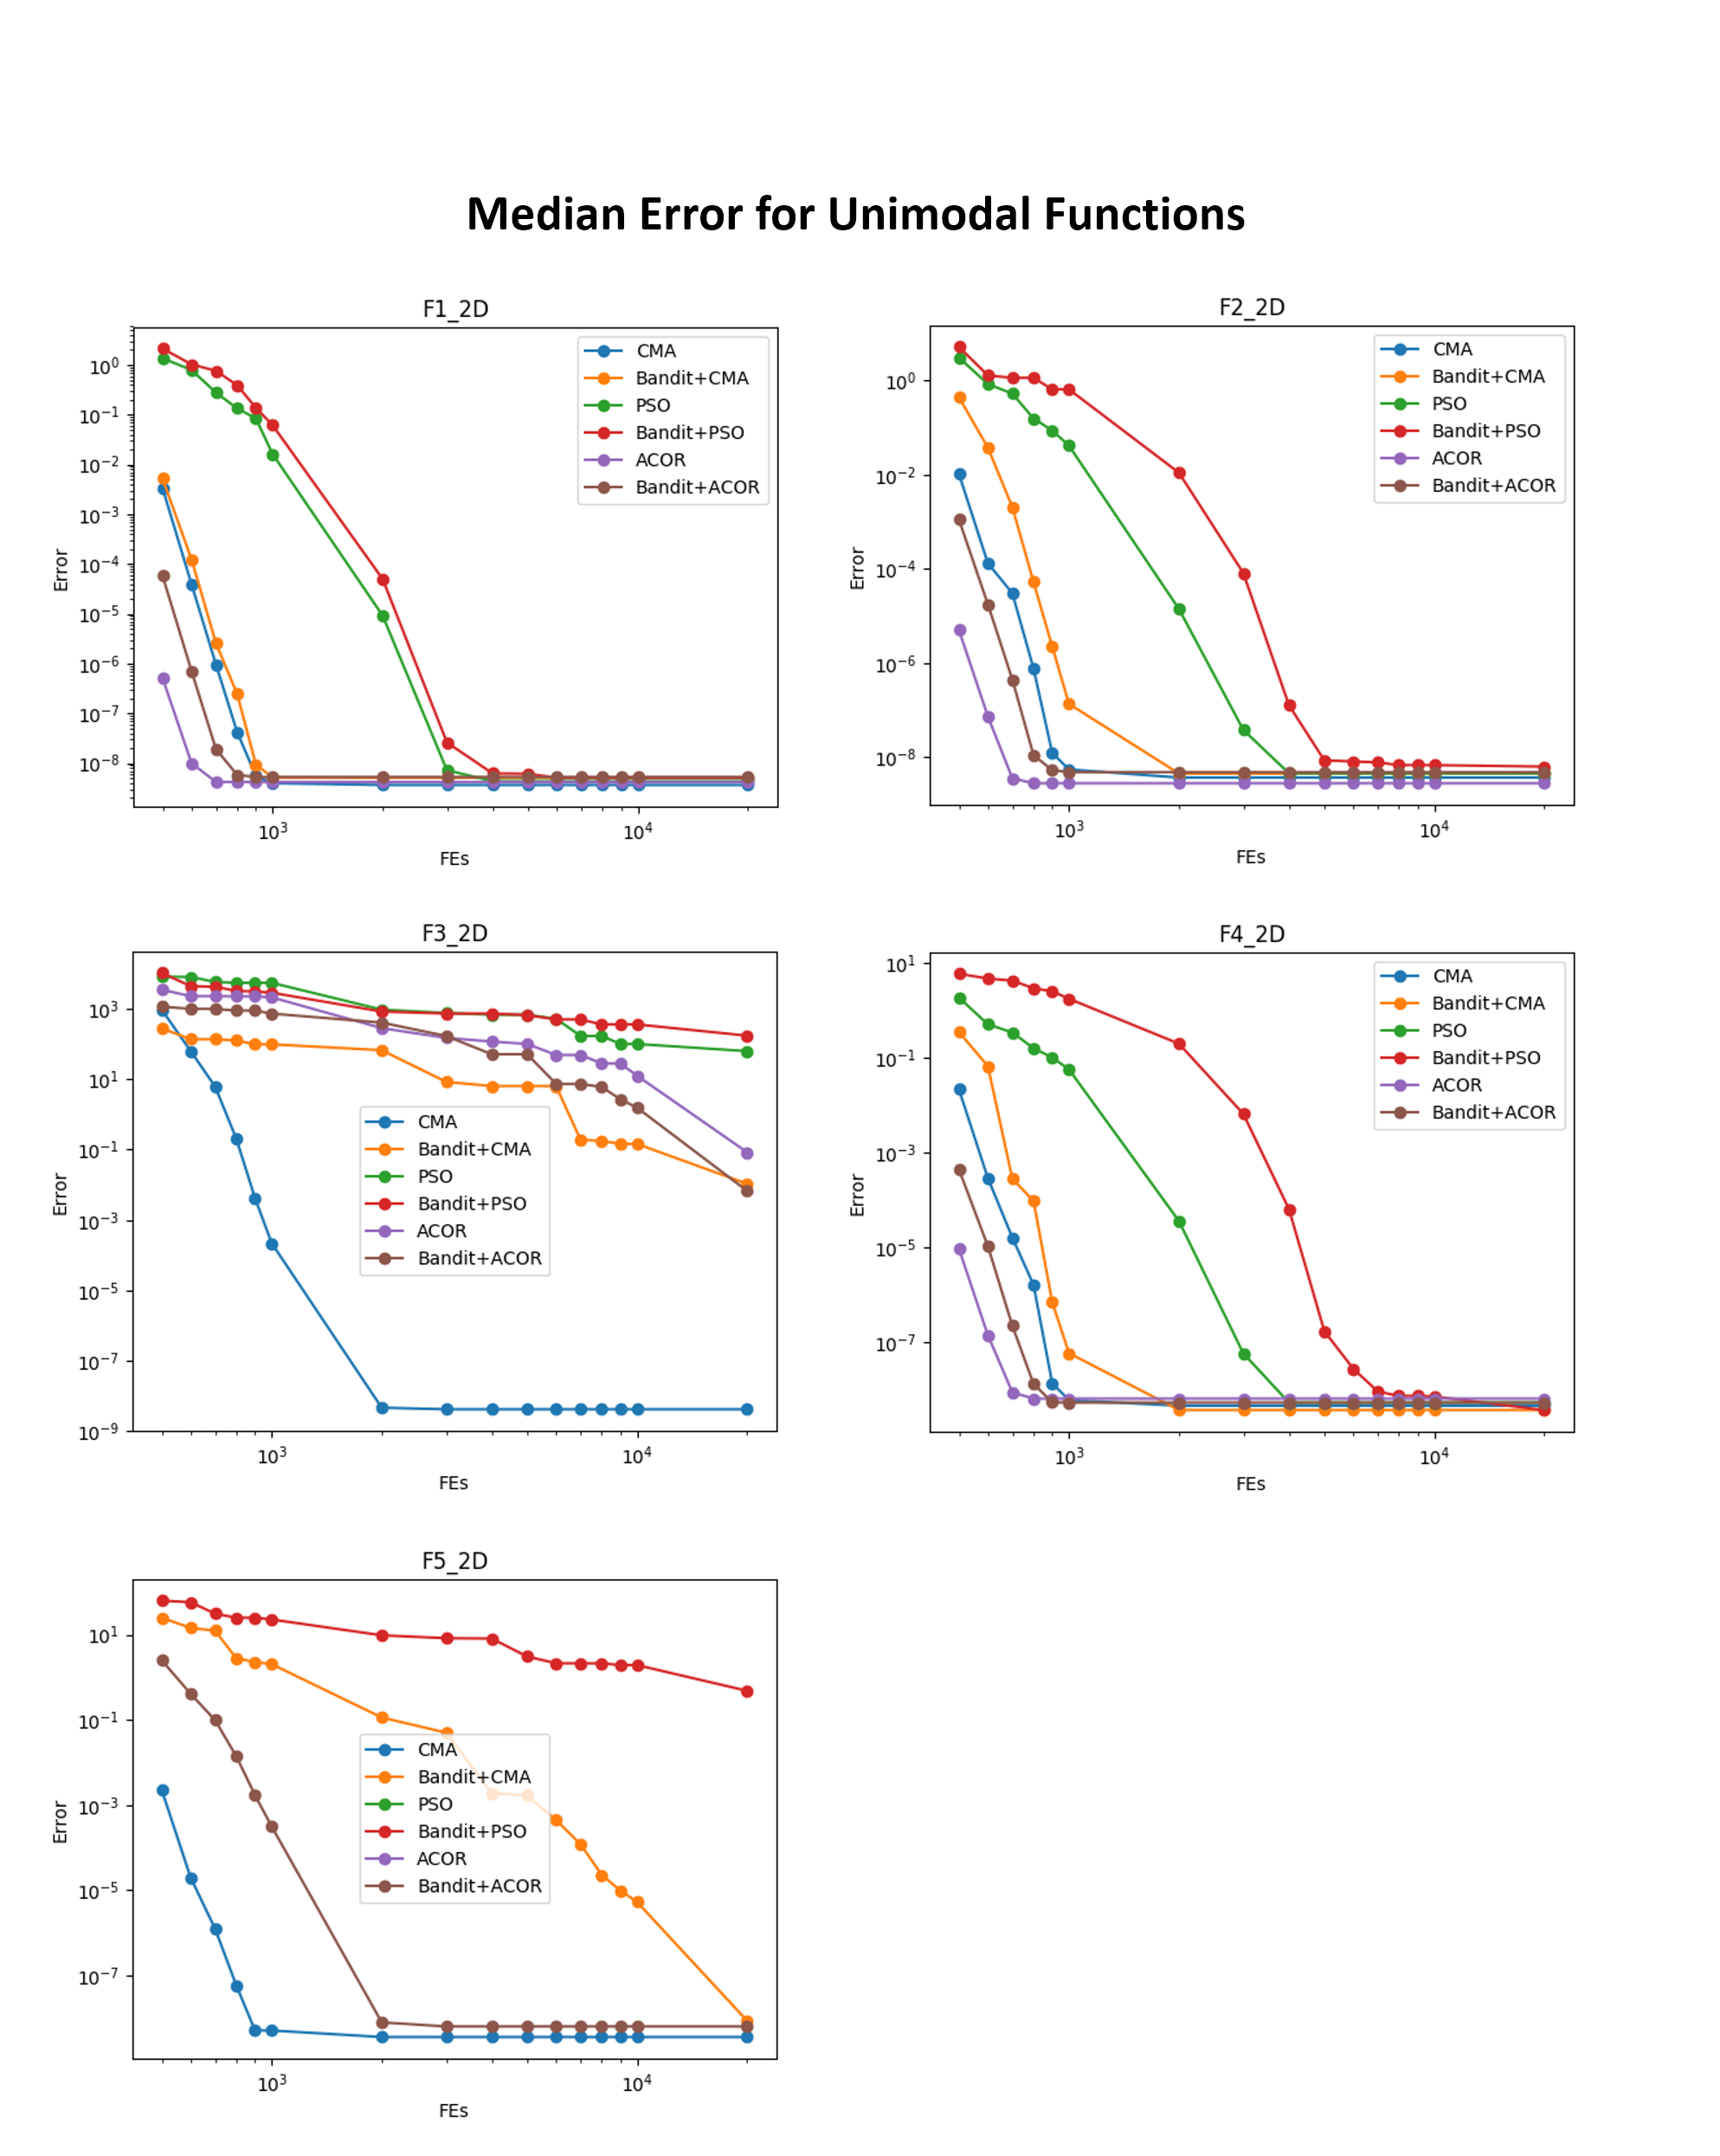
\includegraphics[width=\textwidth]{Median_F1_F5}
%\caption{Median Error for Unimodal Functions.}\label{fig:Median_F1_F5}
%\end{figure} 
%
%\begin{figure}
%\centering
%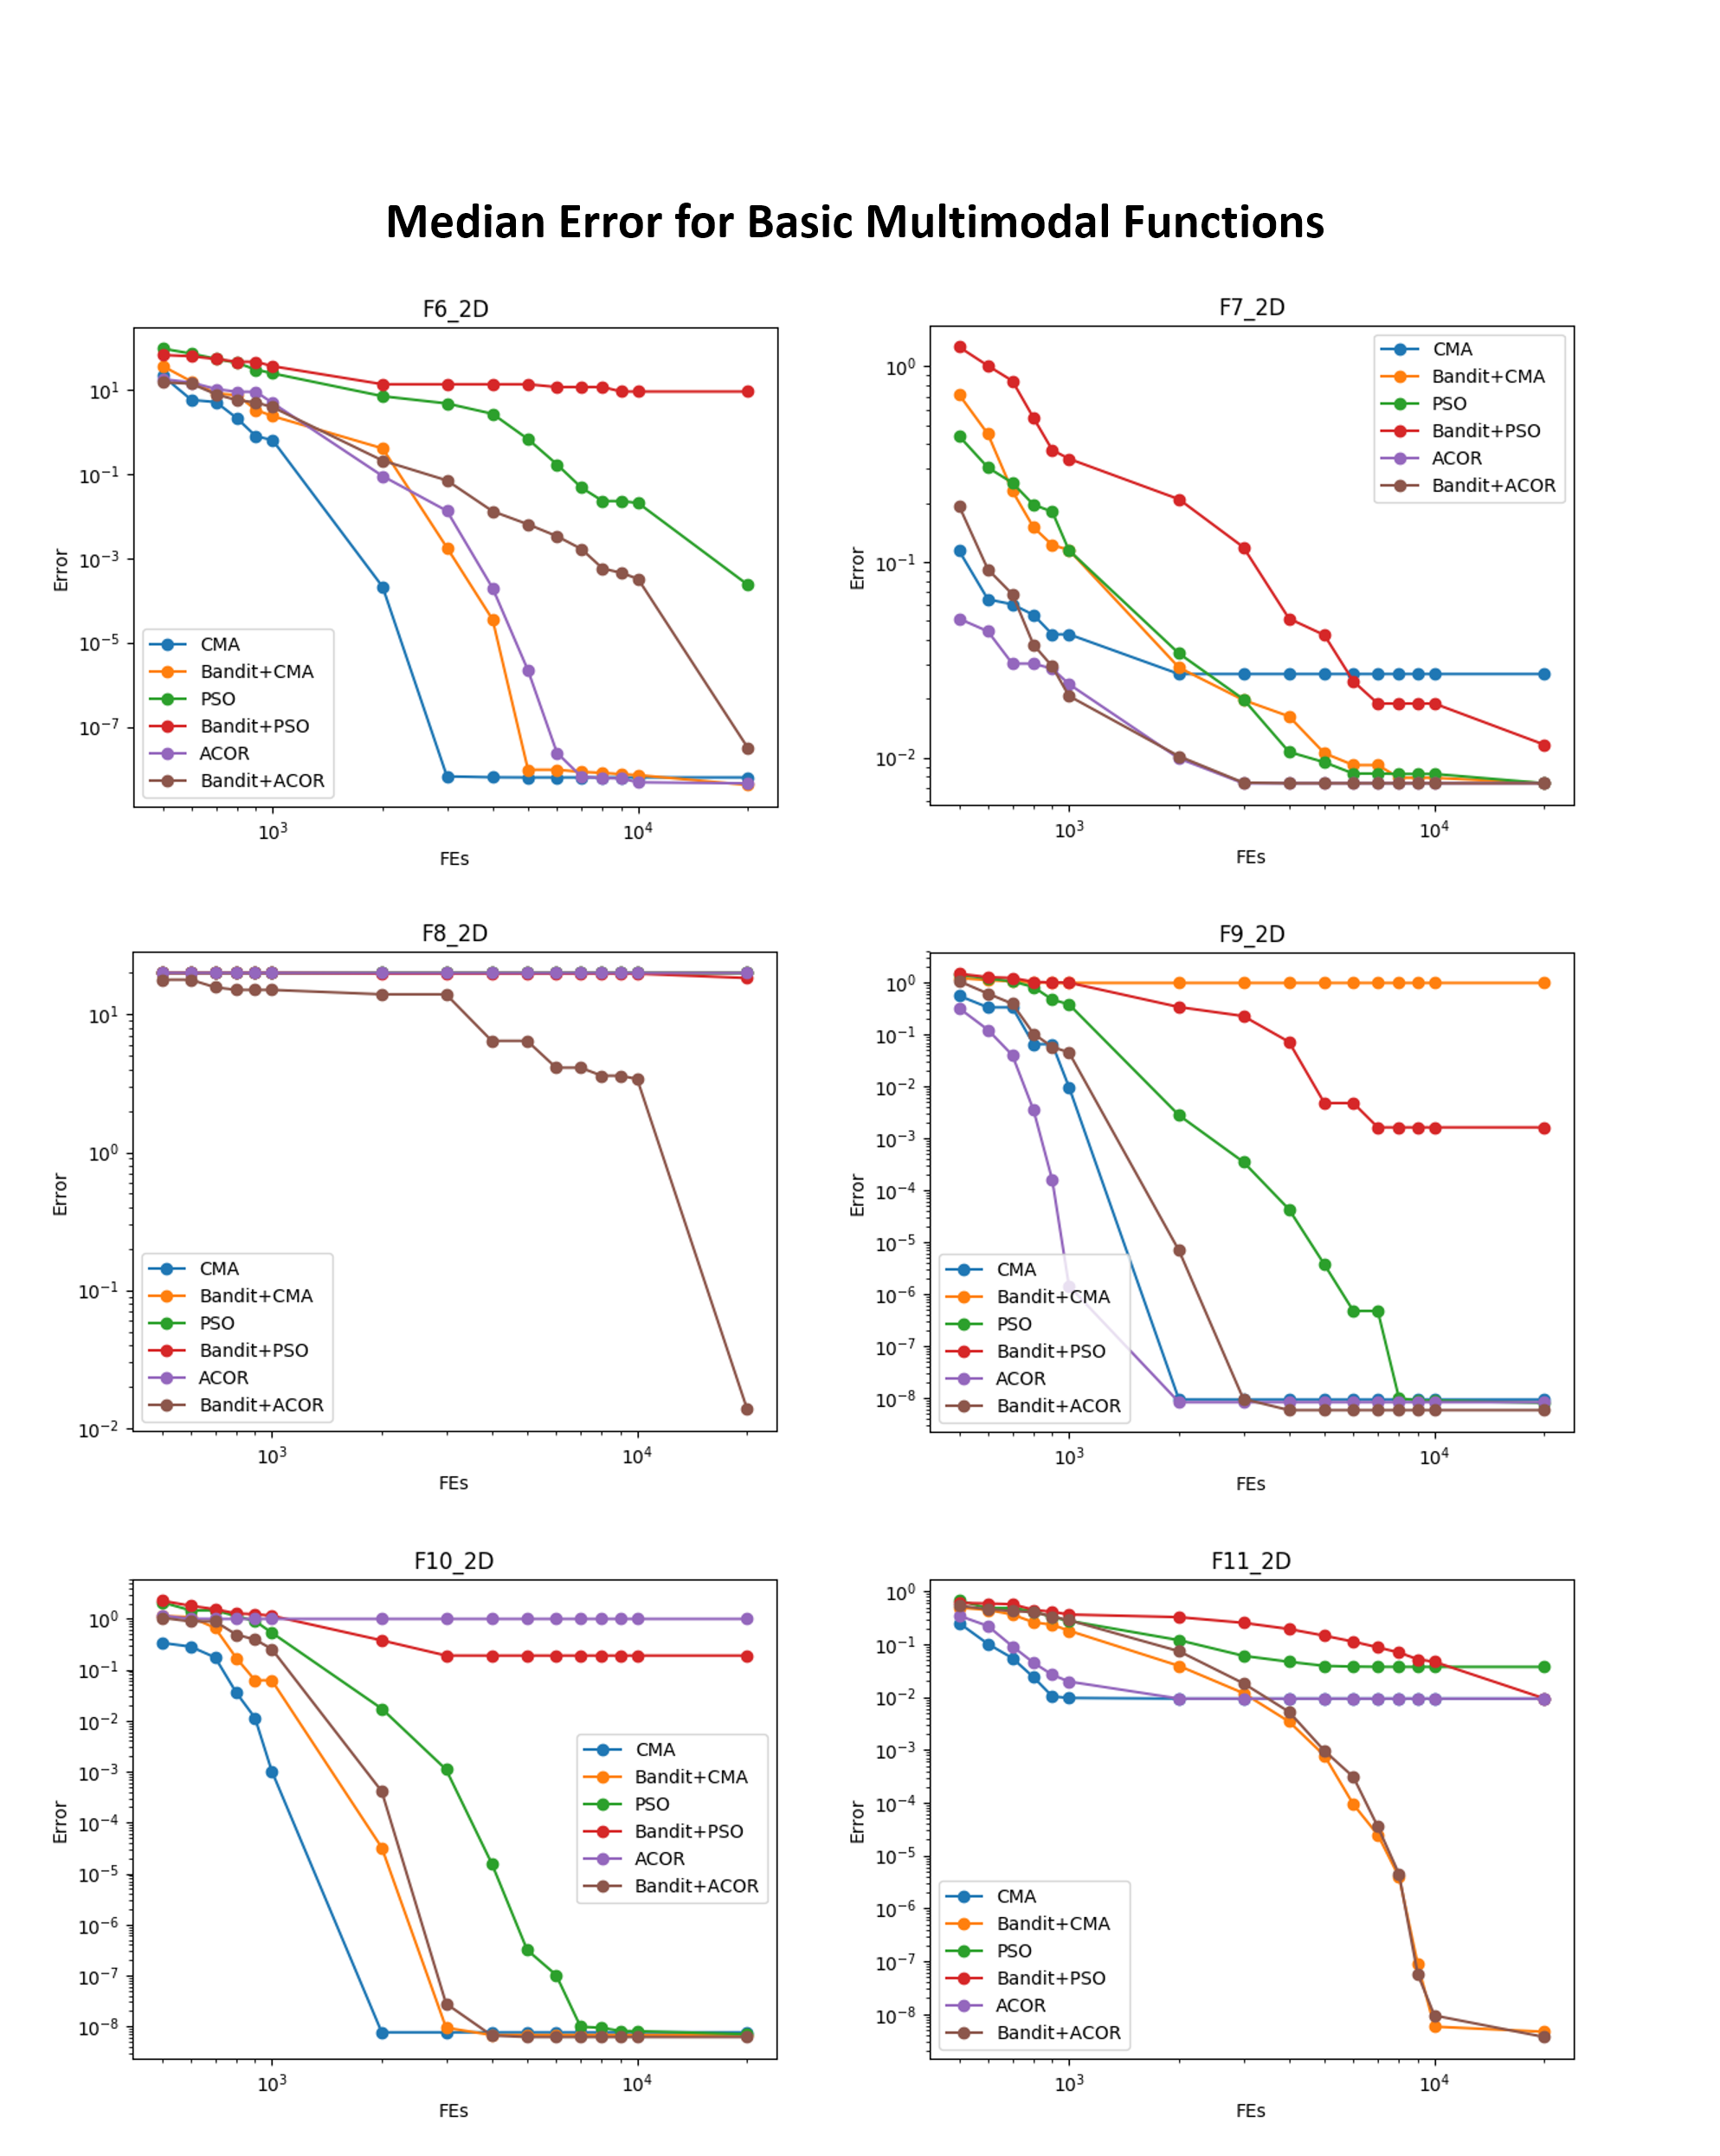
\includegraphics[width=\textwidth]{Median_F6_F11}
%\caption{Median Error for Basic Multimodal Functions.}\label{fig:Median_F6_F11}
%\end{figure} 
%
%\begin{figure}
%\centering
%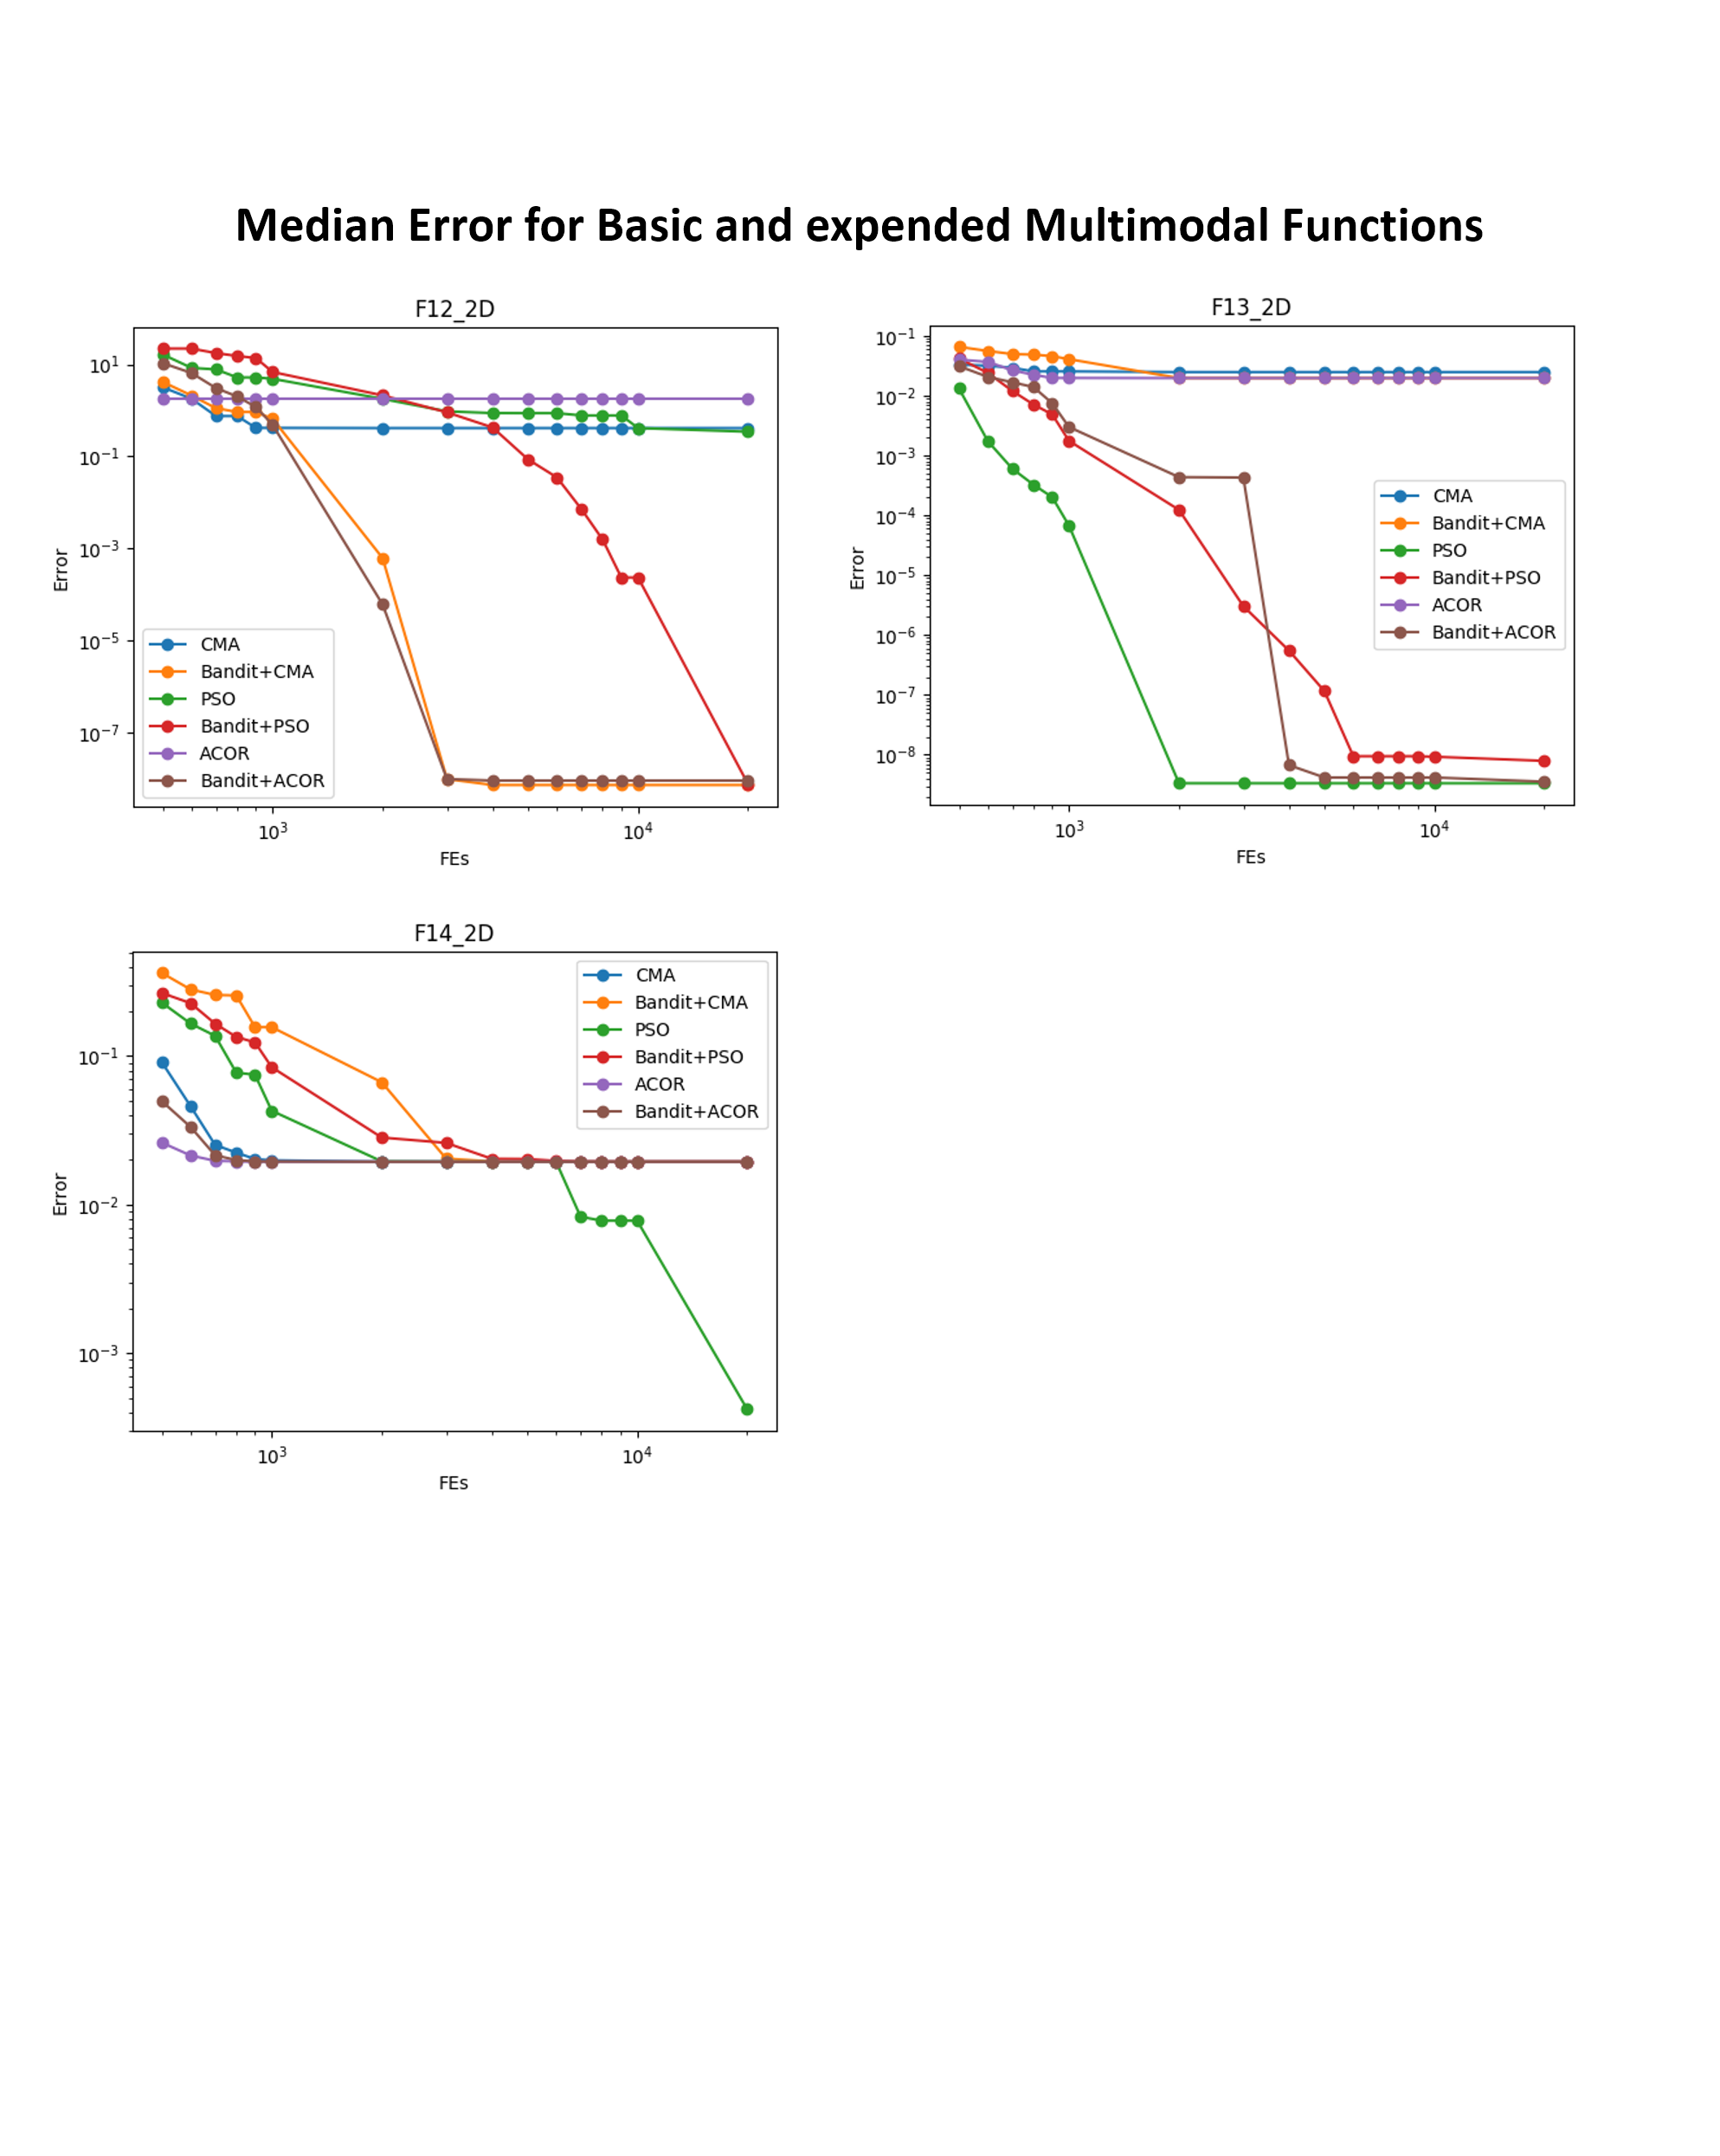
\includegraphics[width=\textwidth]{Median_F12_F14}
%\caption{Median Error for Basic and expended Functions.}\label{fig:Median_F12_F14}
%\end{figure} 
%
%\begin{figure}
%\centering
%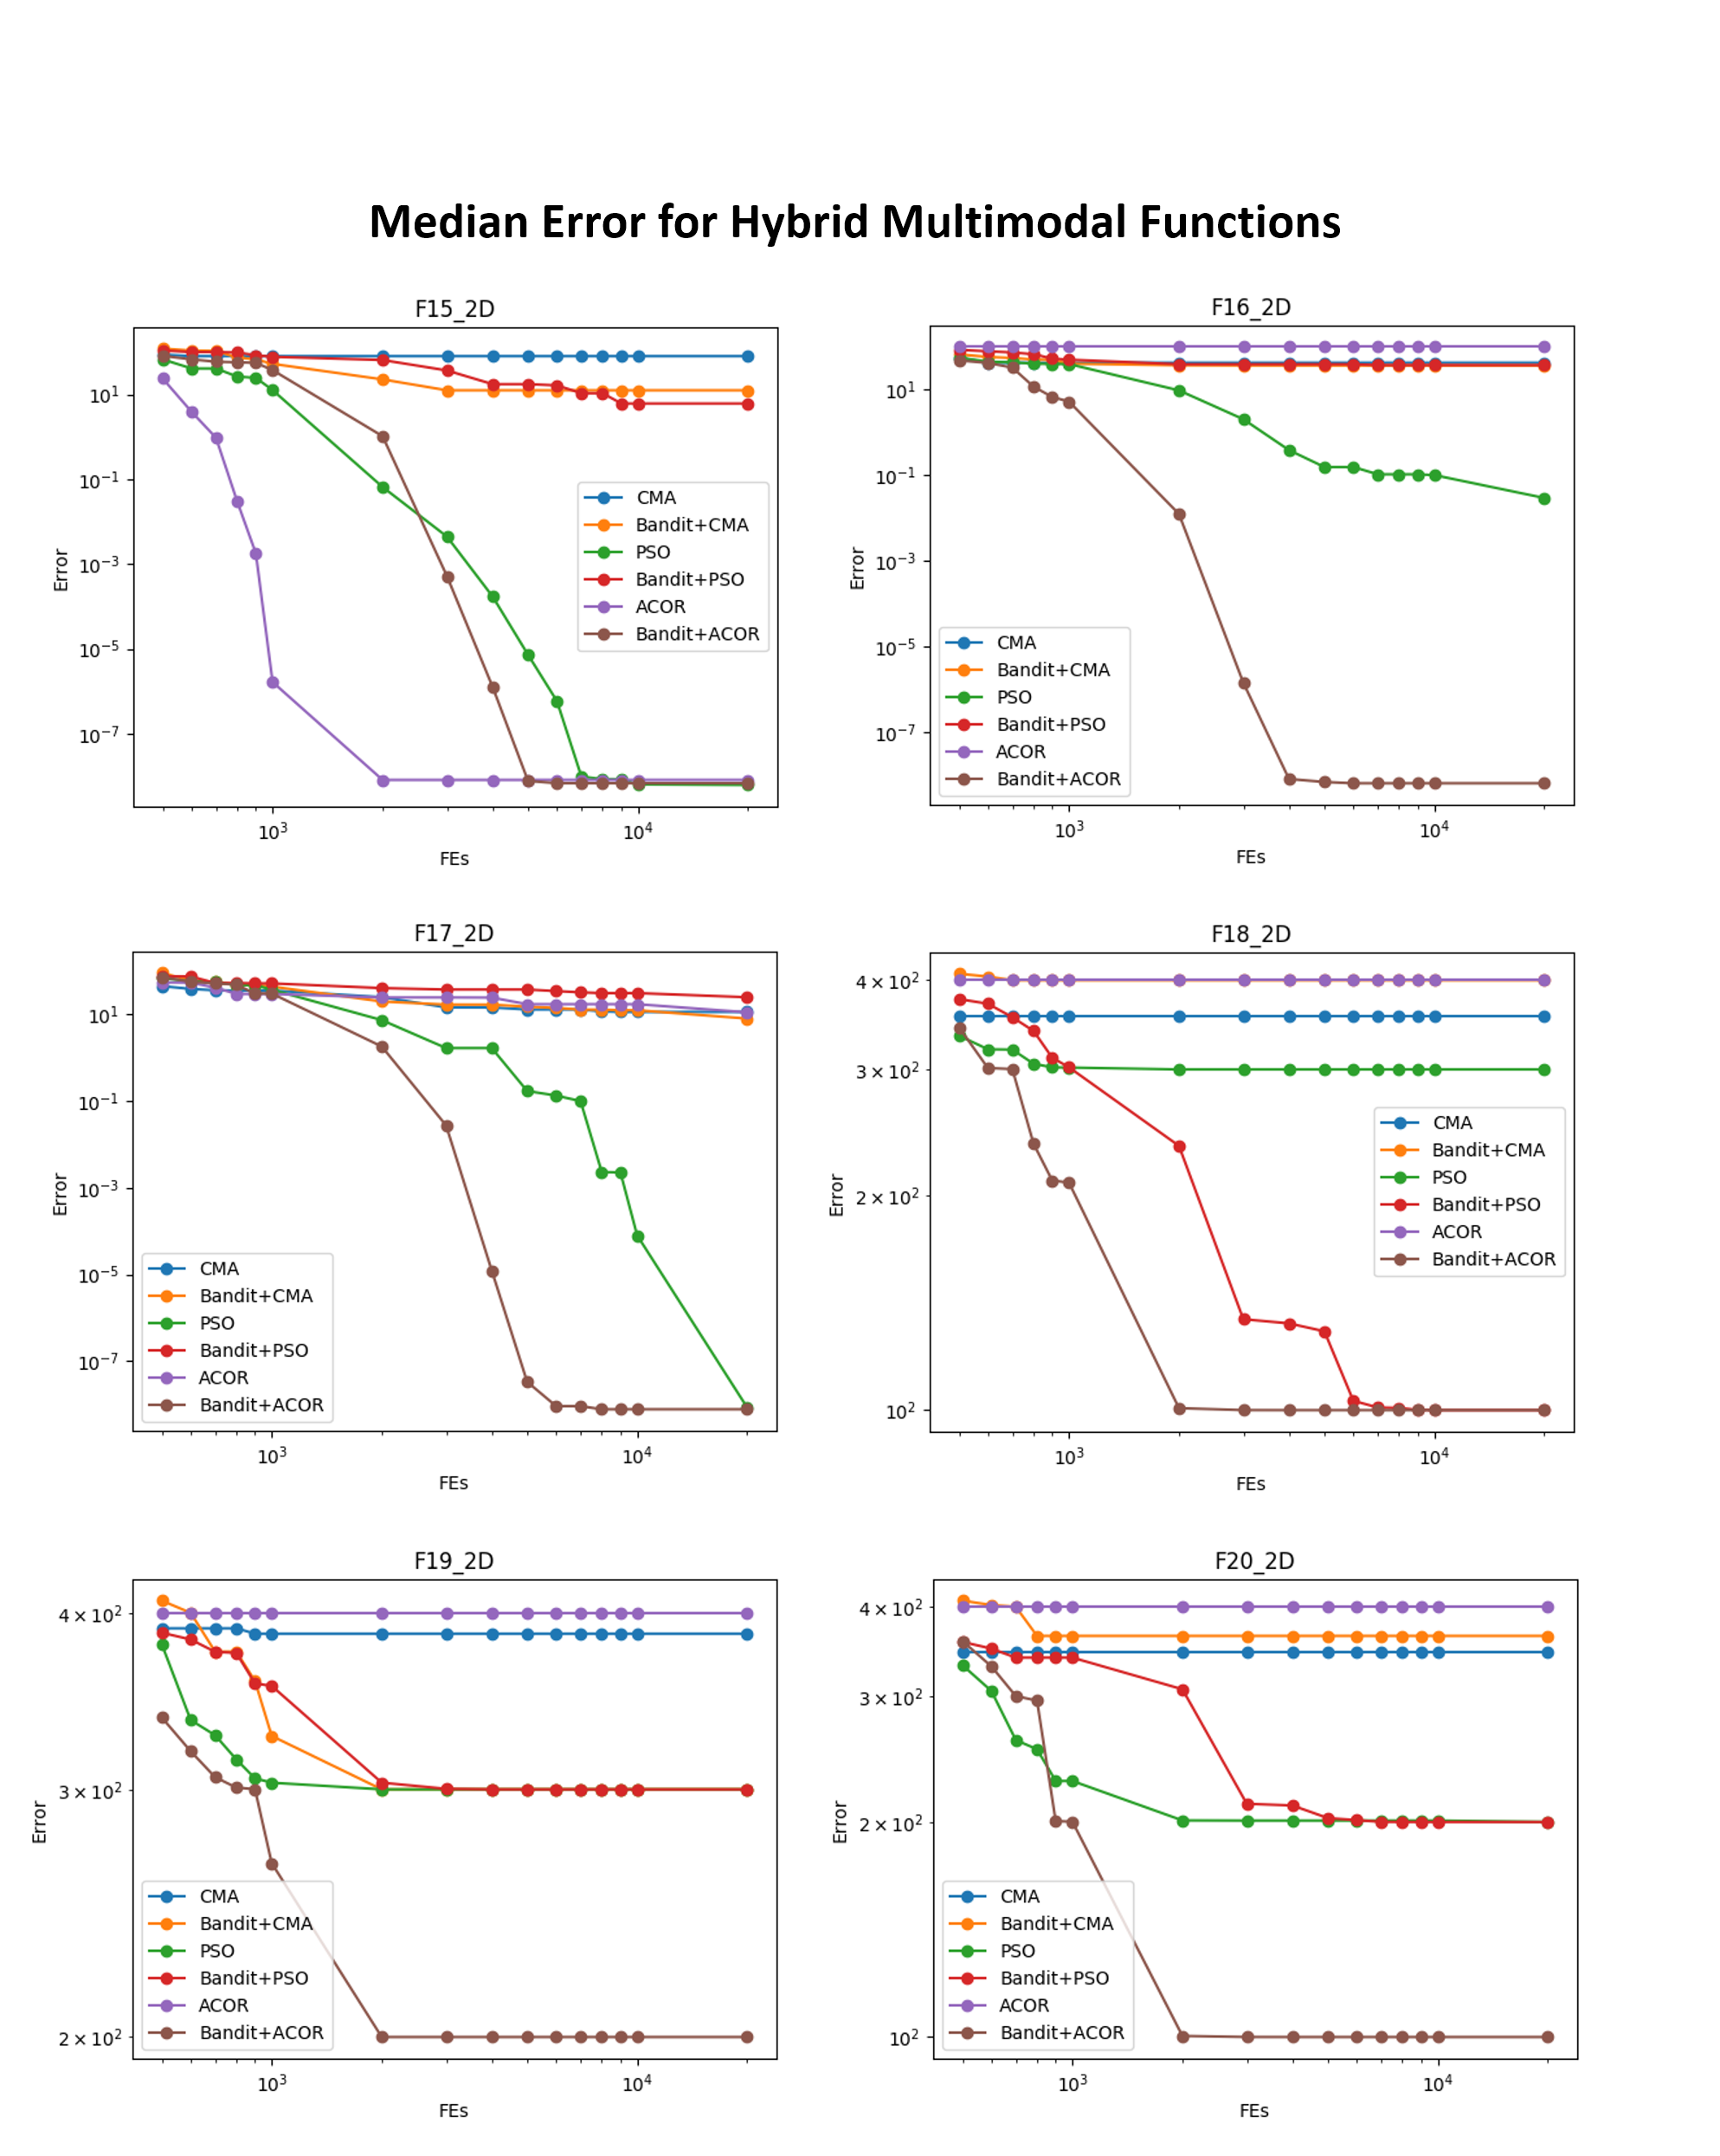
\includegraphics[width=\textwidth]{Median_F15_F20}
%\caption{Median Error for Hybrid Multimodal Functions.}\label{fig:Median_F15_F20}
%\end{figure} 
%
%\begin{figure}
%\centering
%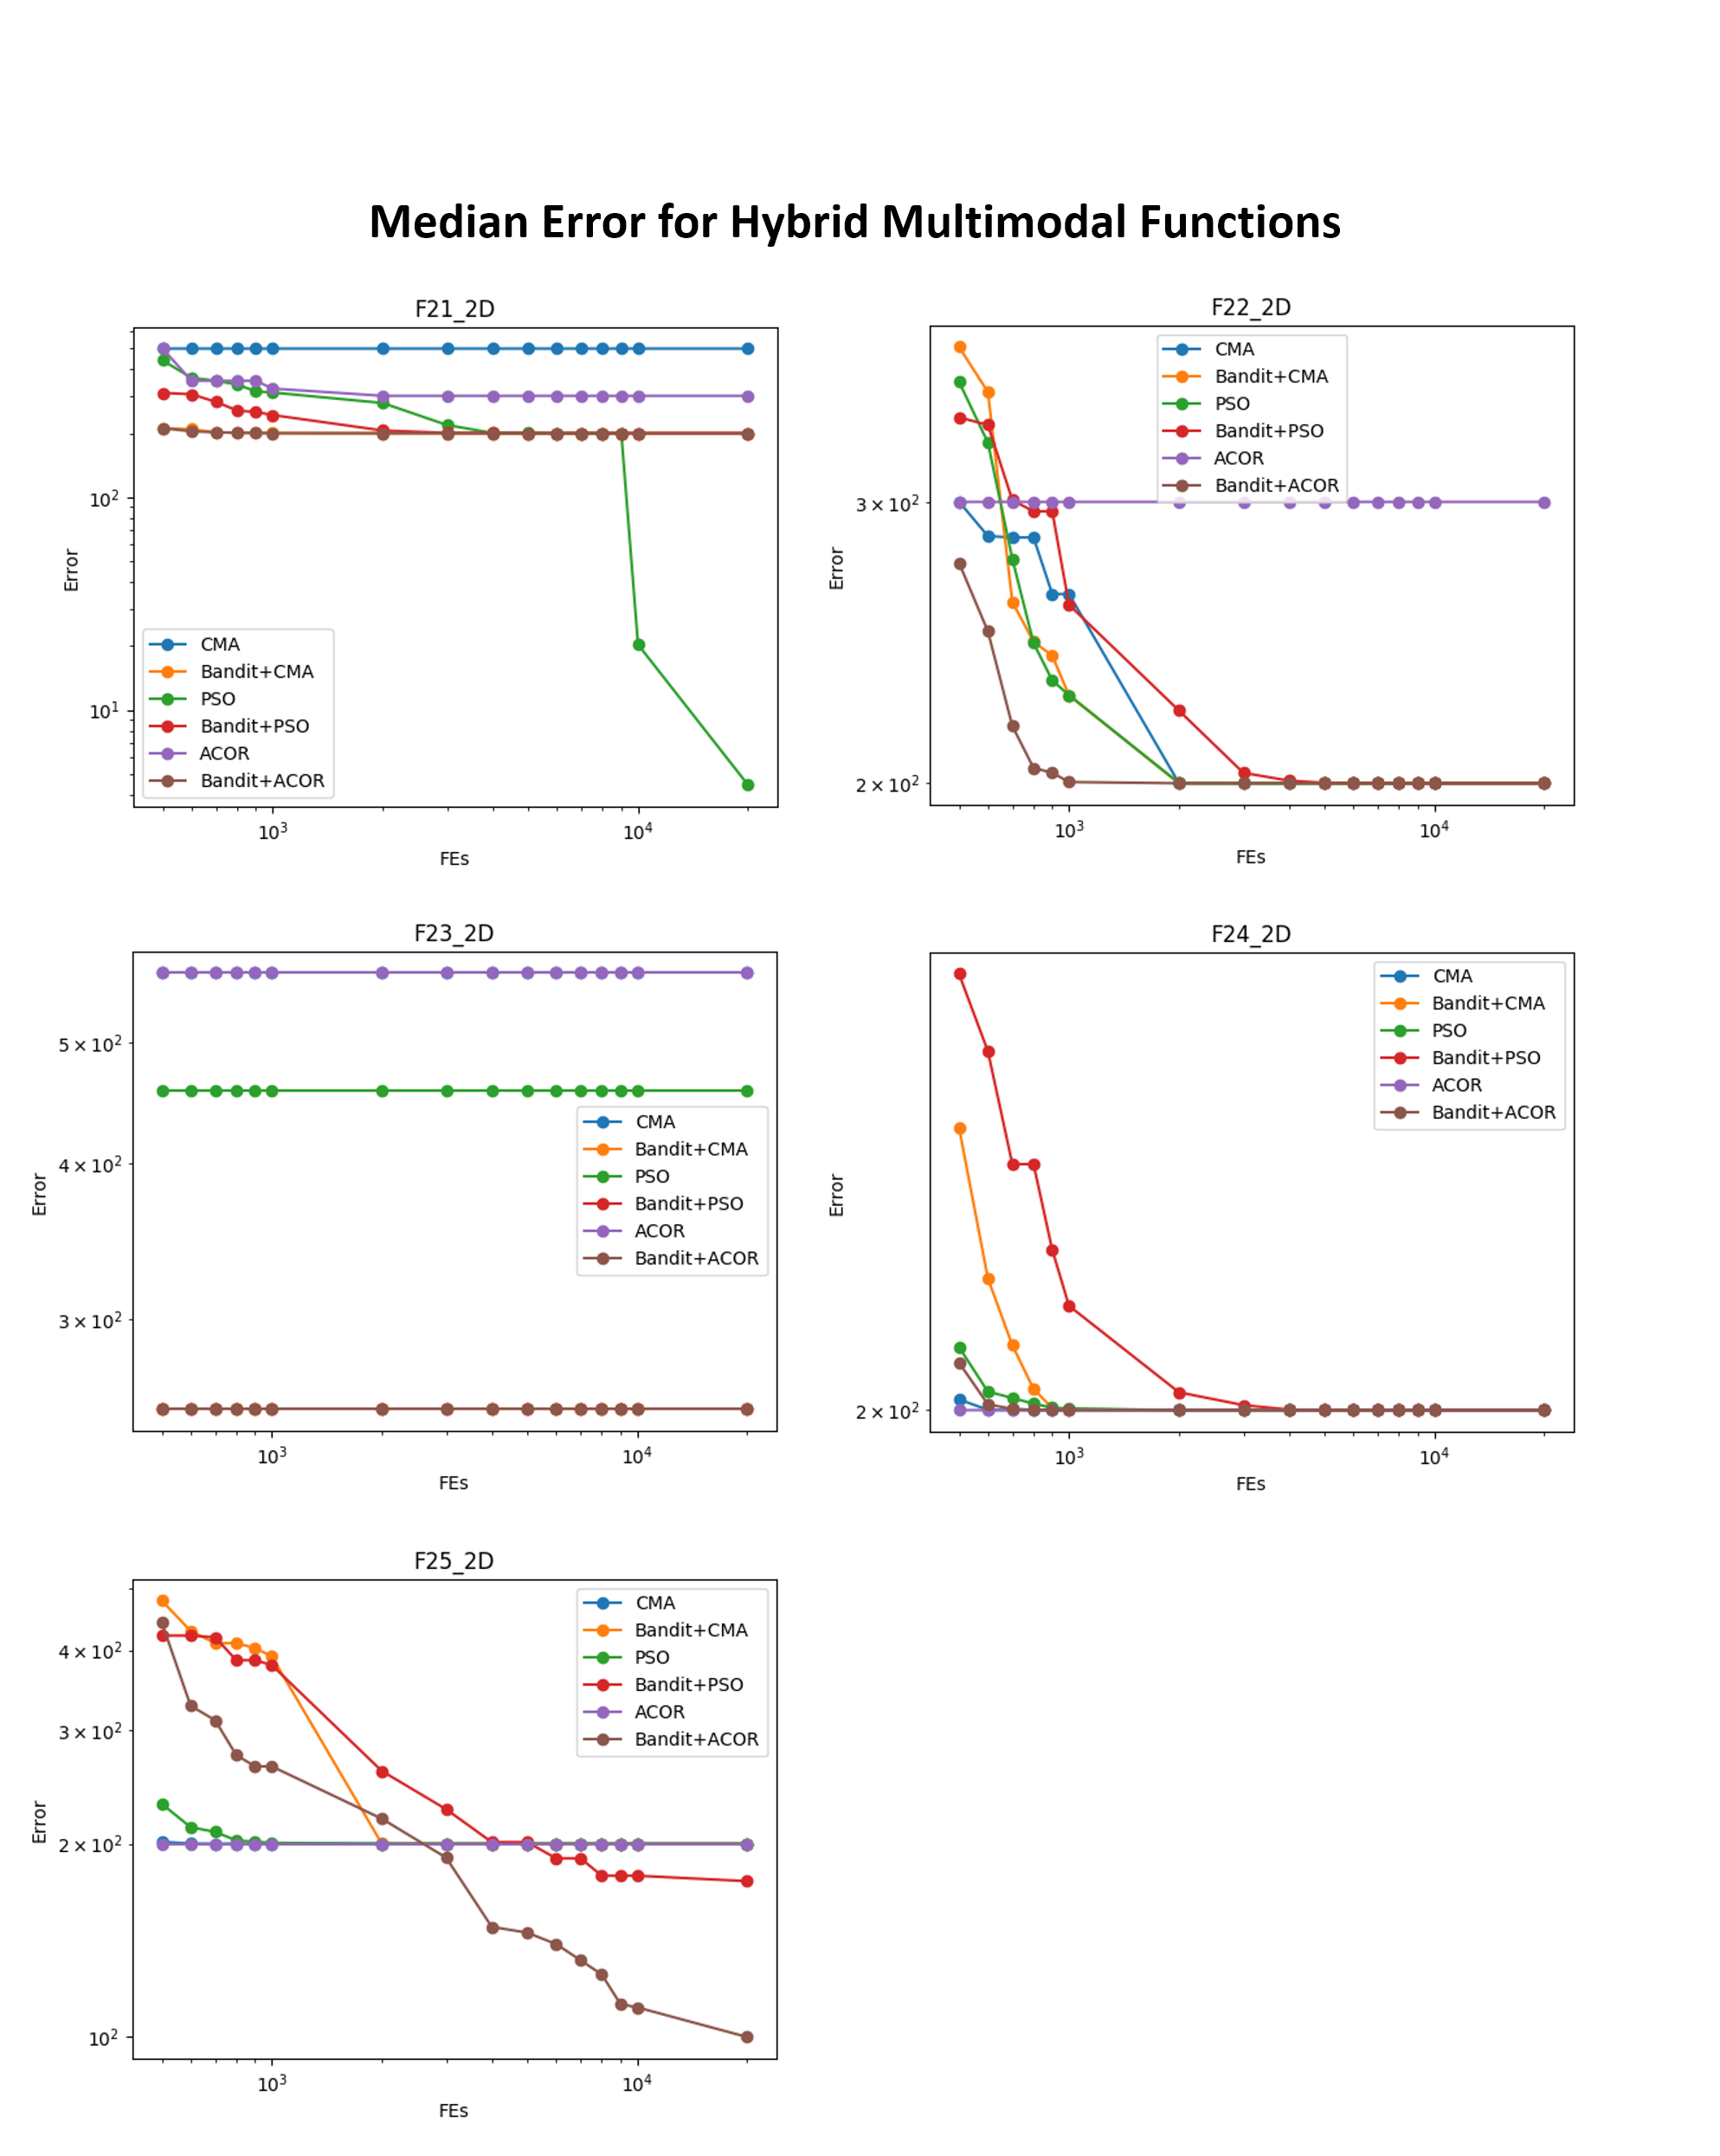
\includegraphics[width=\textwidth]{Median_F21_F25}
%\caption{Median Error for Hybrid Multimodal Functions.}\label{fig:Median_F21_F25}
%\end{figure} 
%
%\begin{figure}
%\centering
%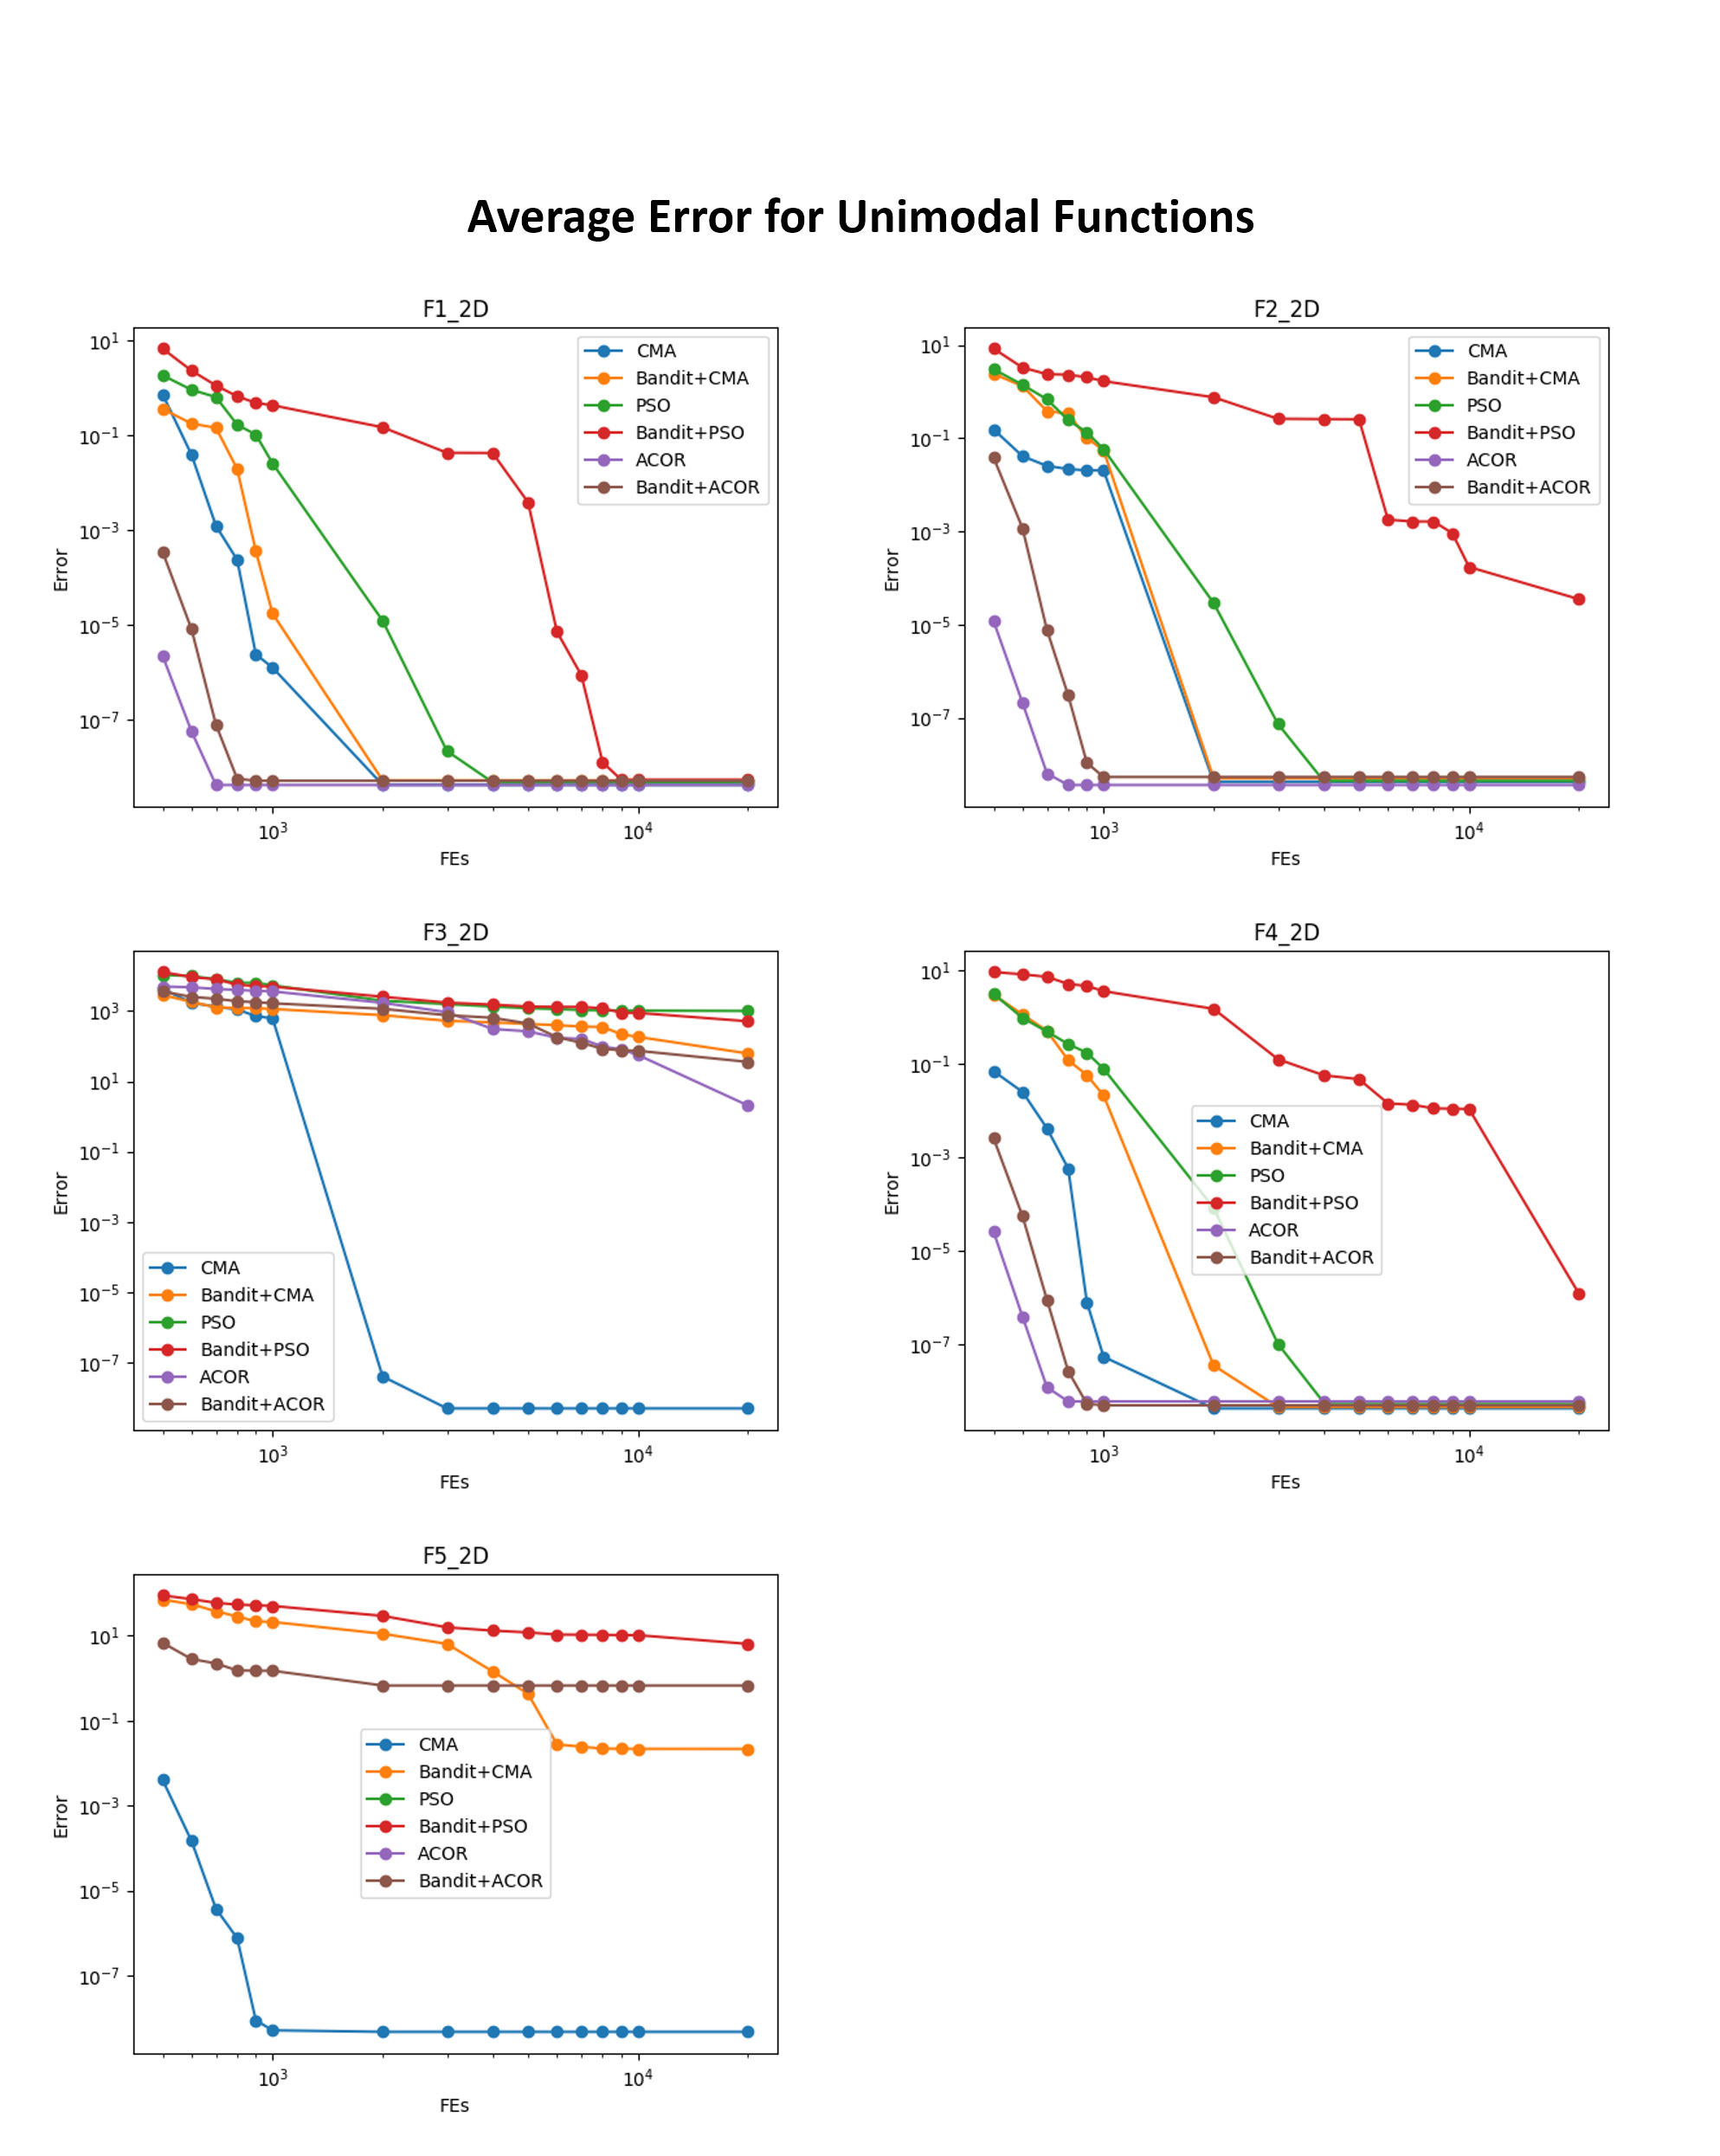
\includegraphics[width=\textwidth]{Average_F1_F5}
%\caption{Average Error for Unimodal Functions.}\label{fig:Average_F1_F5}
%\end{figure} 
%
%\begin{figure}
%\centering
%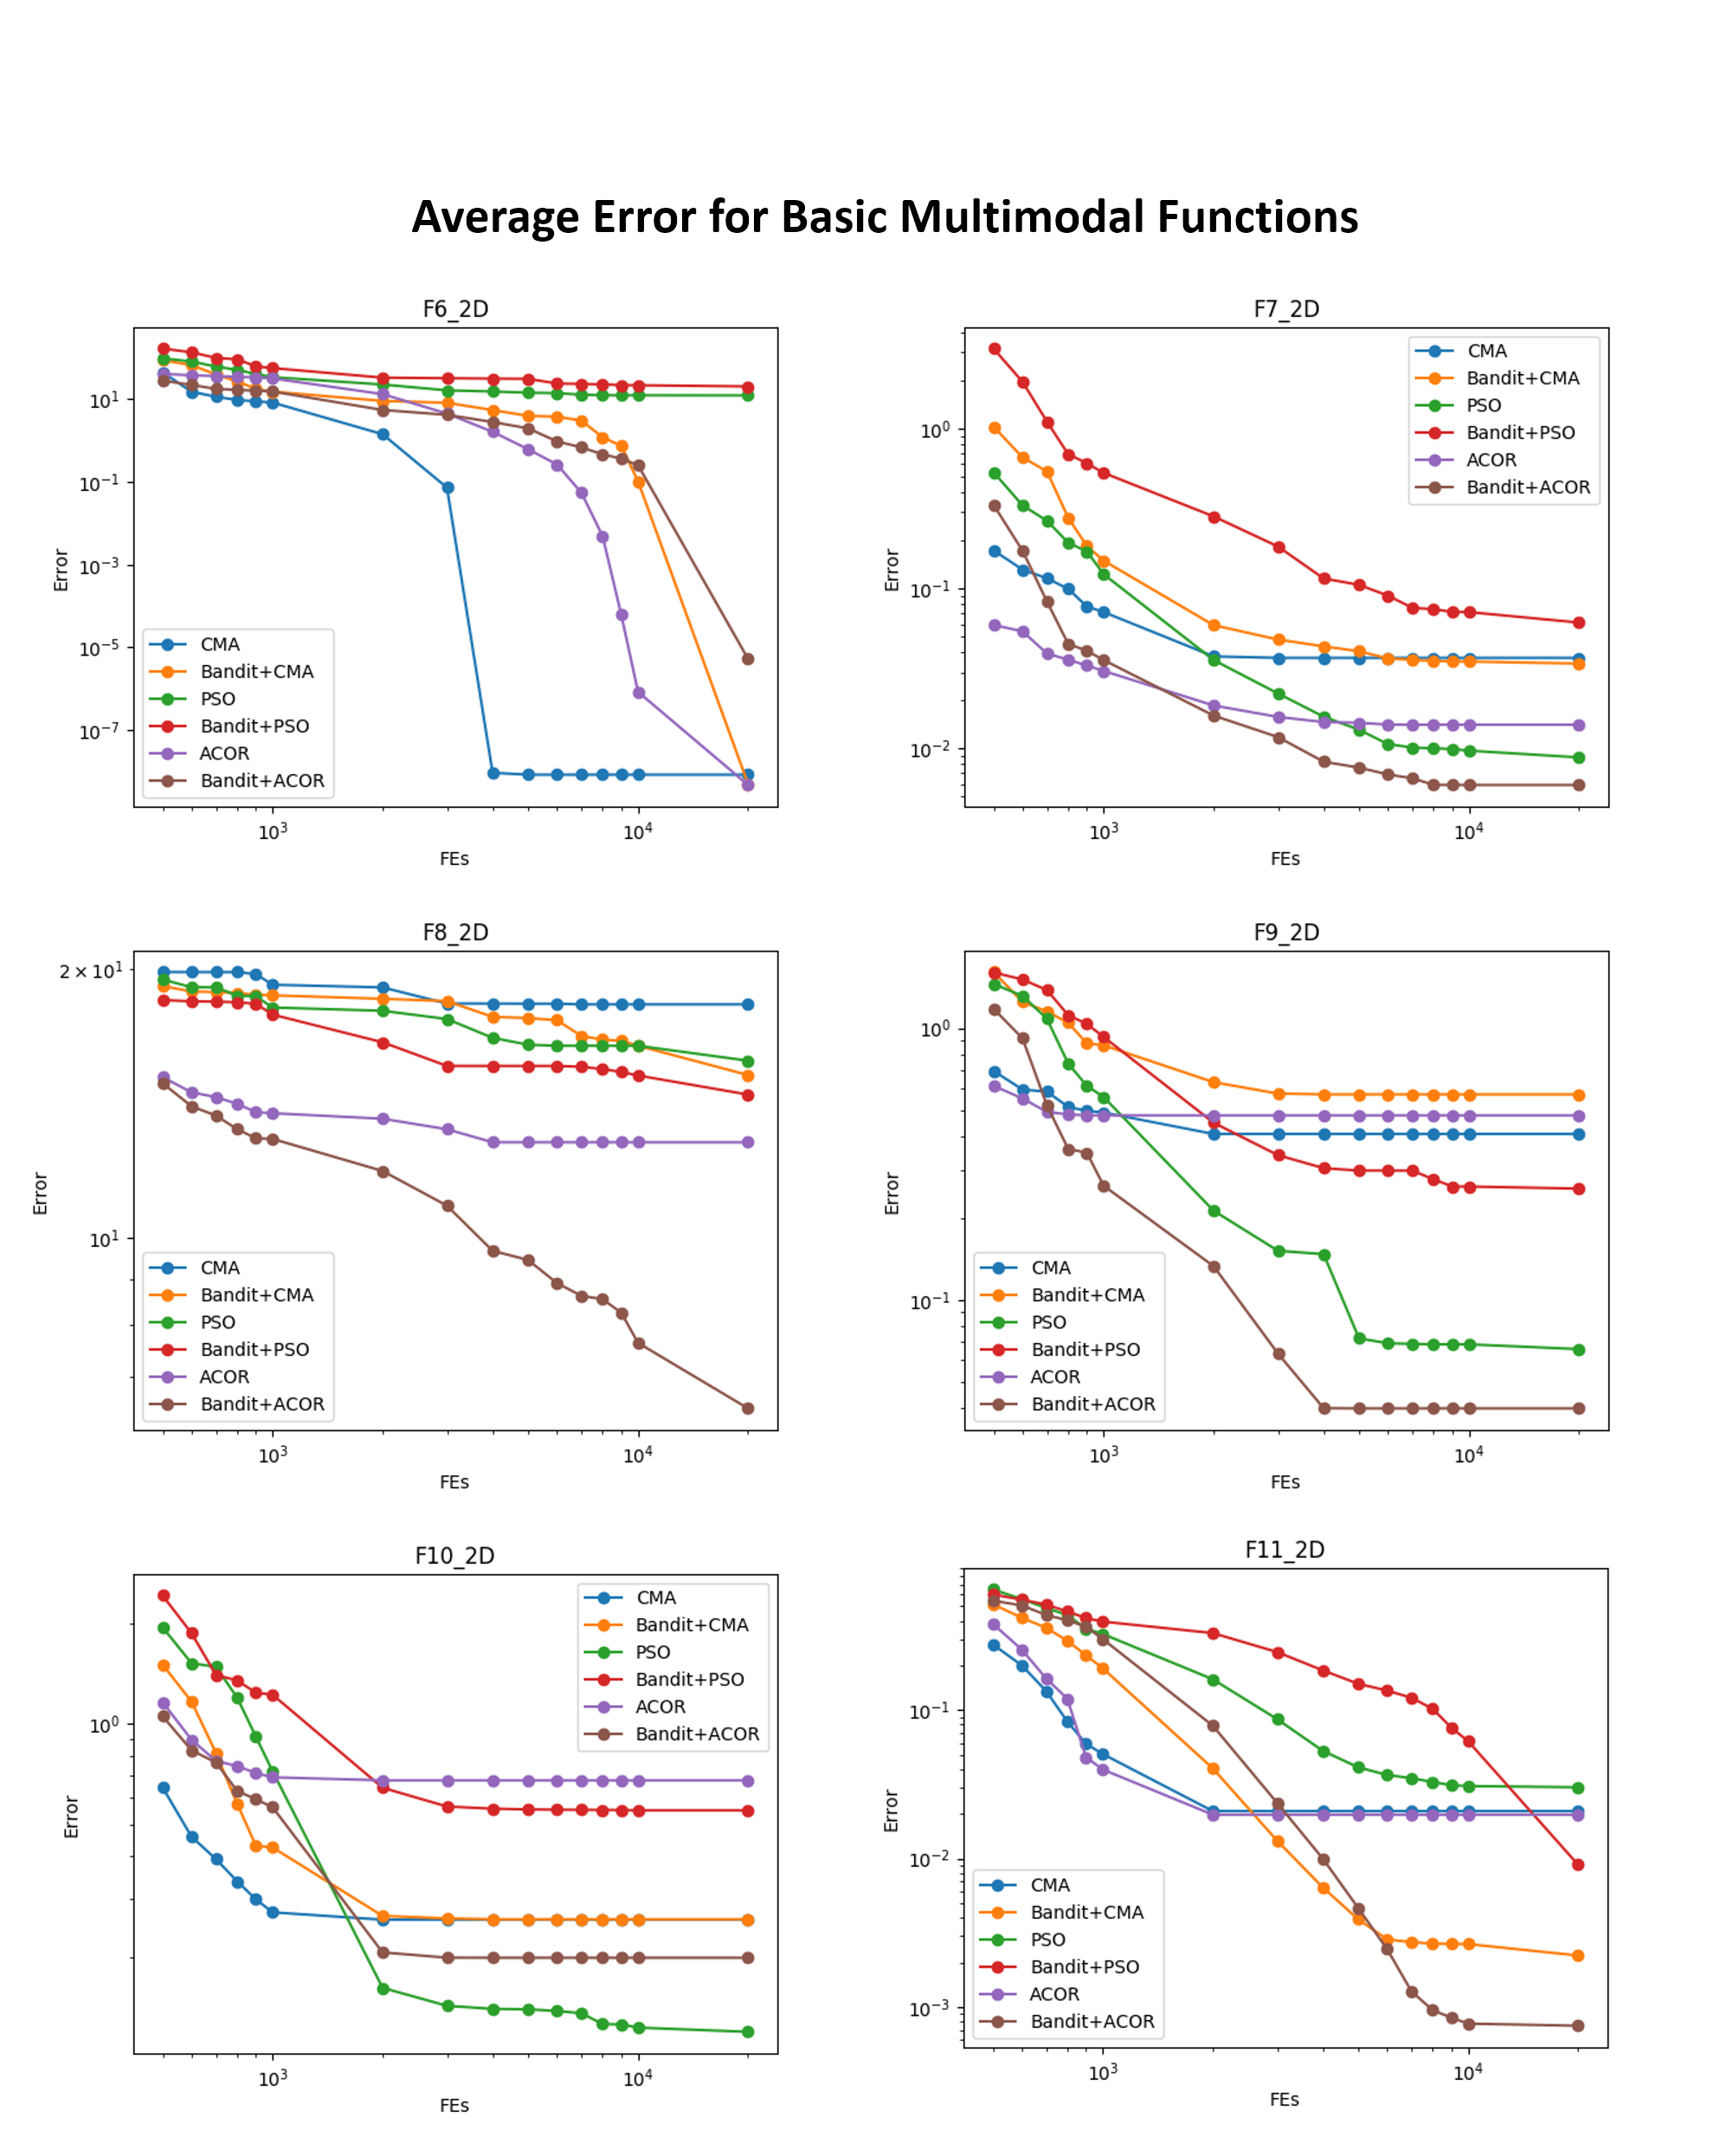
\includegraphics[width=\textwidth]{Average_F6_F11}
%\caption{Average Error for Basic Multimodal Functions.}\label{fig:Average_F6_F11}
%\end{figure} 
%
%\begin{figure}
%\centering
%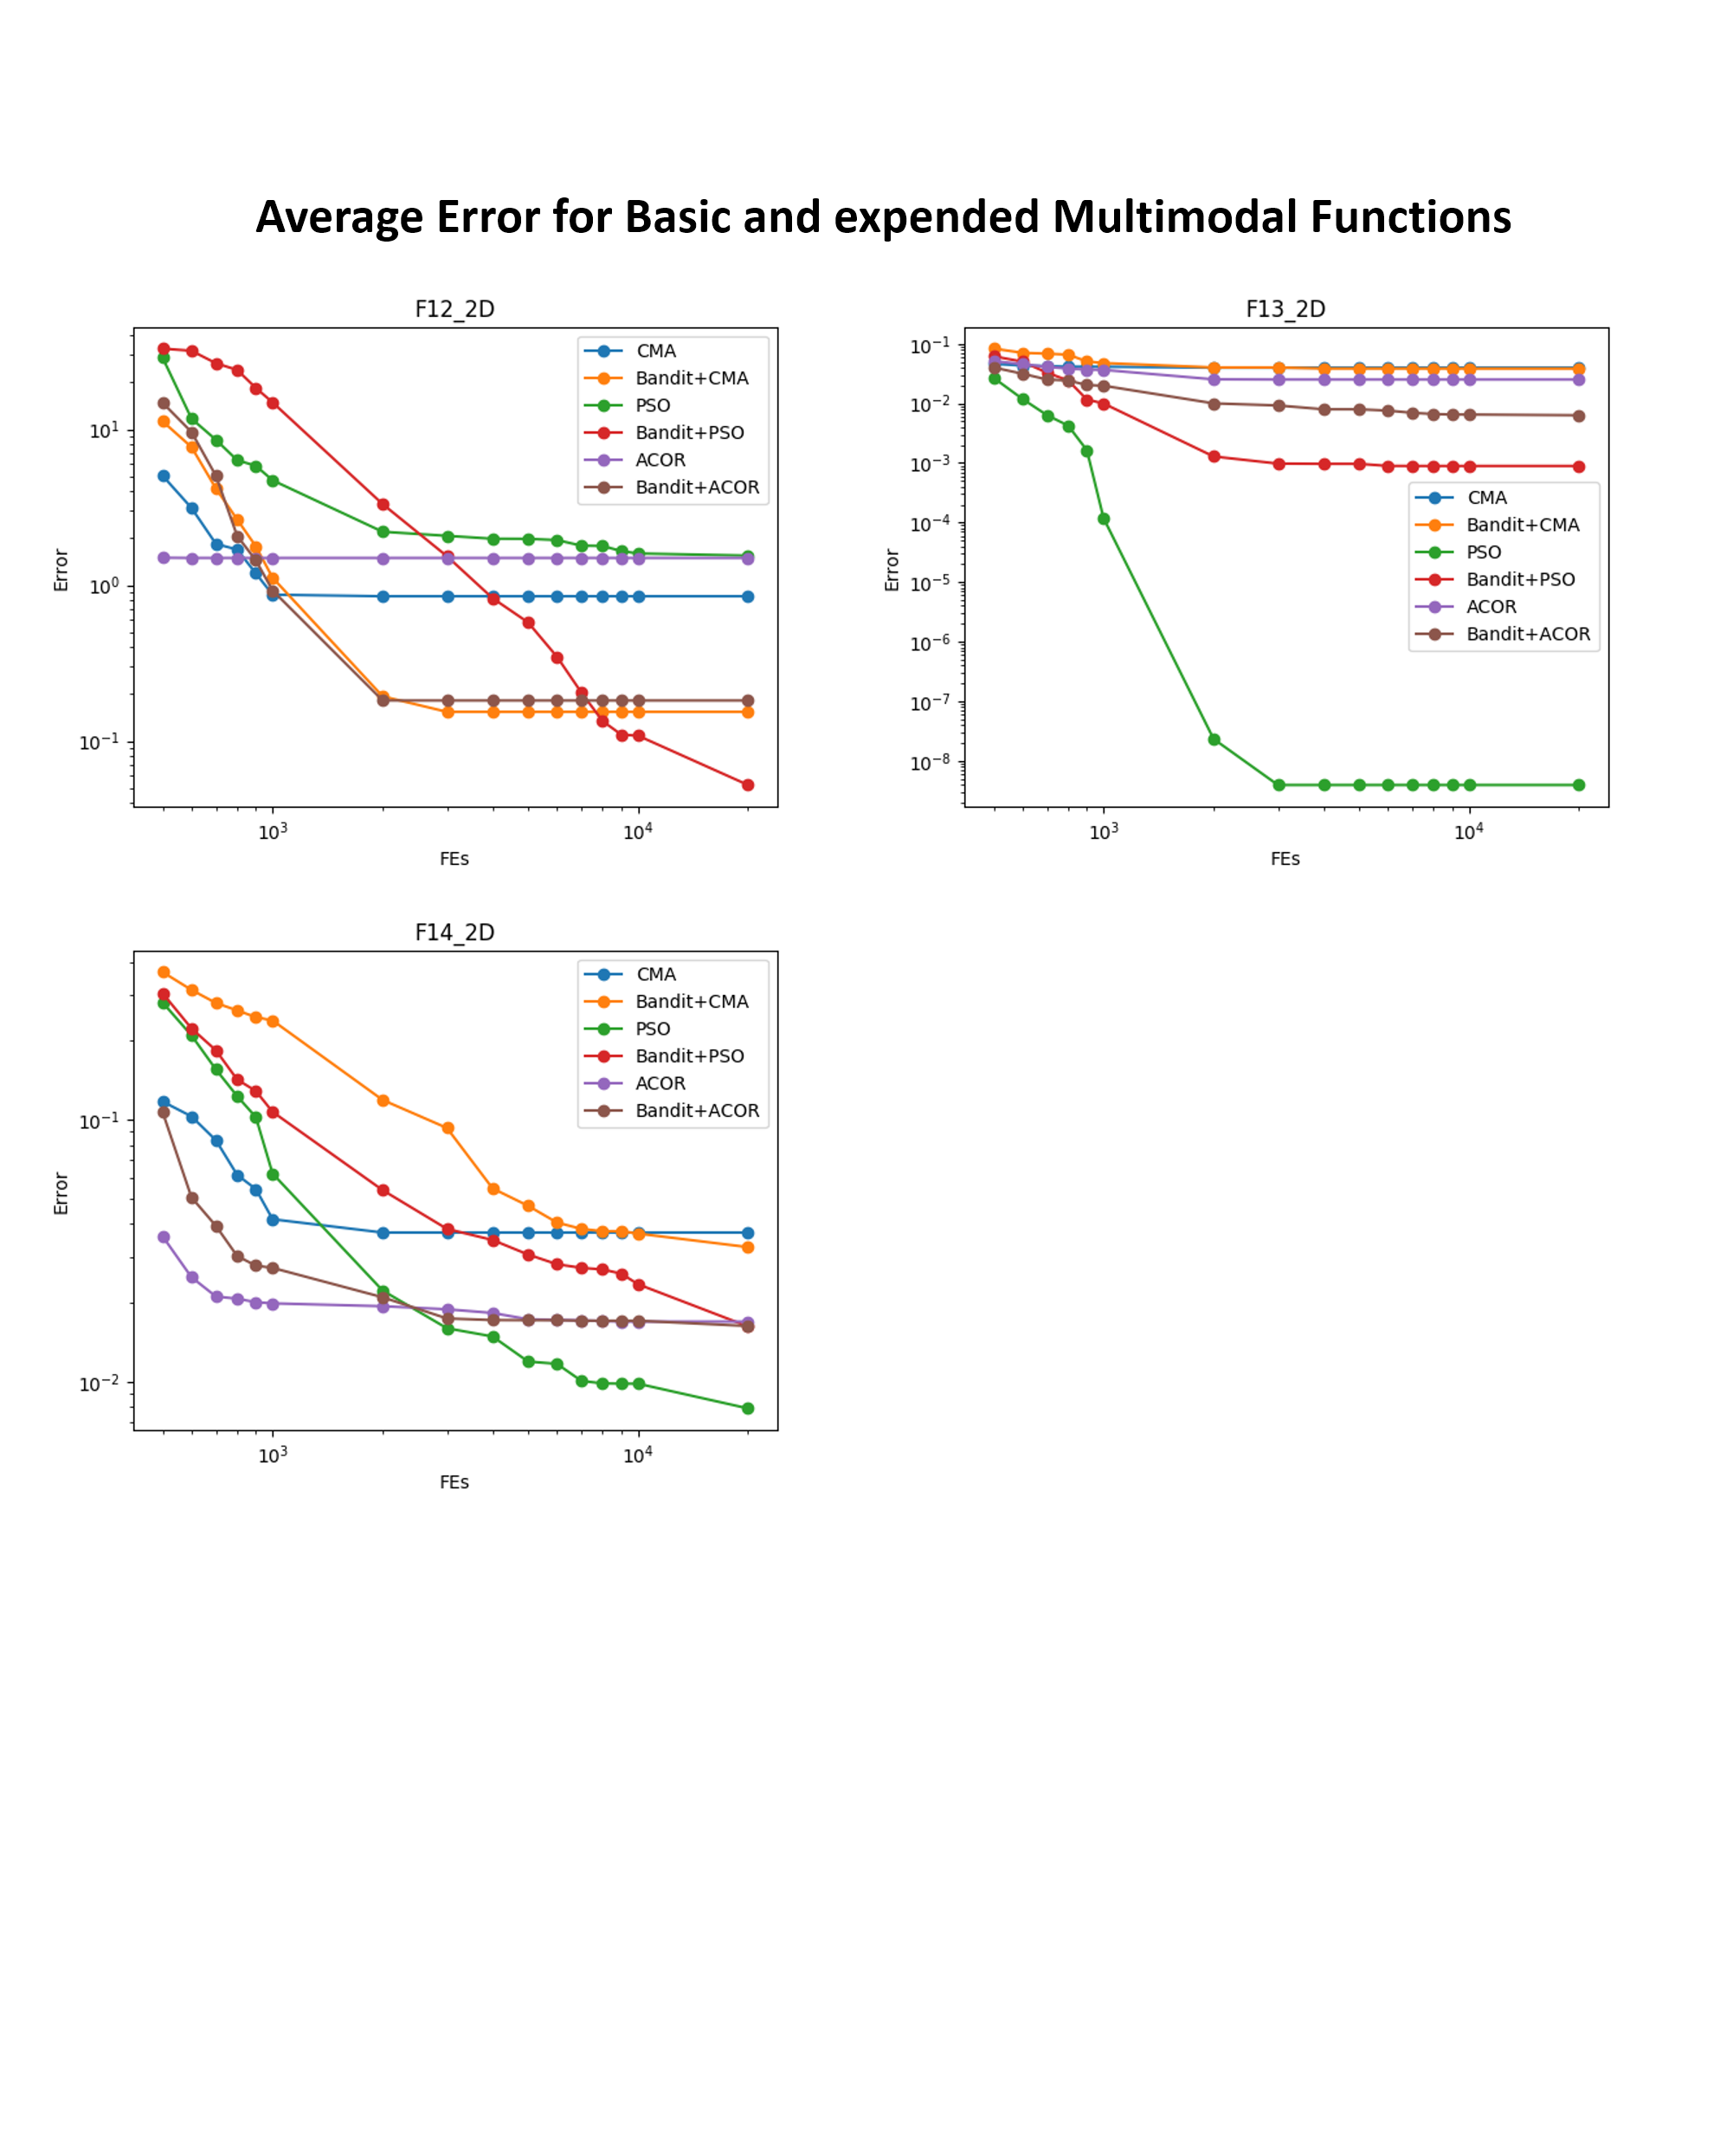
\includegraphics[width=\textwidth]{Average_F12_F14}
%\caption{Average Error for Basic and expended Functions.}\label{fig:Average_F12_F14}
%\end{figure} 
%
%\begin{figure}
%\centering
%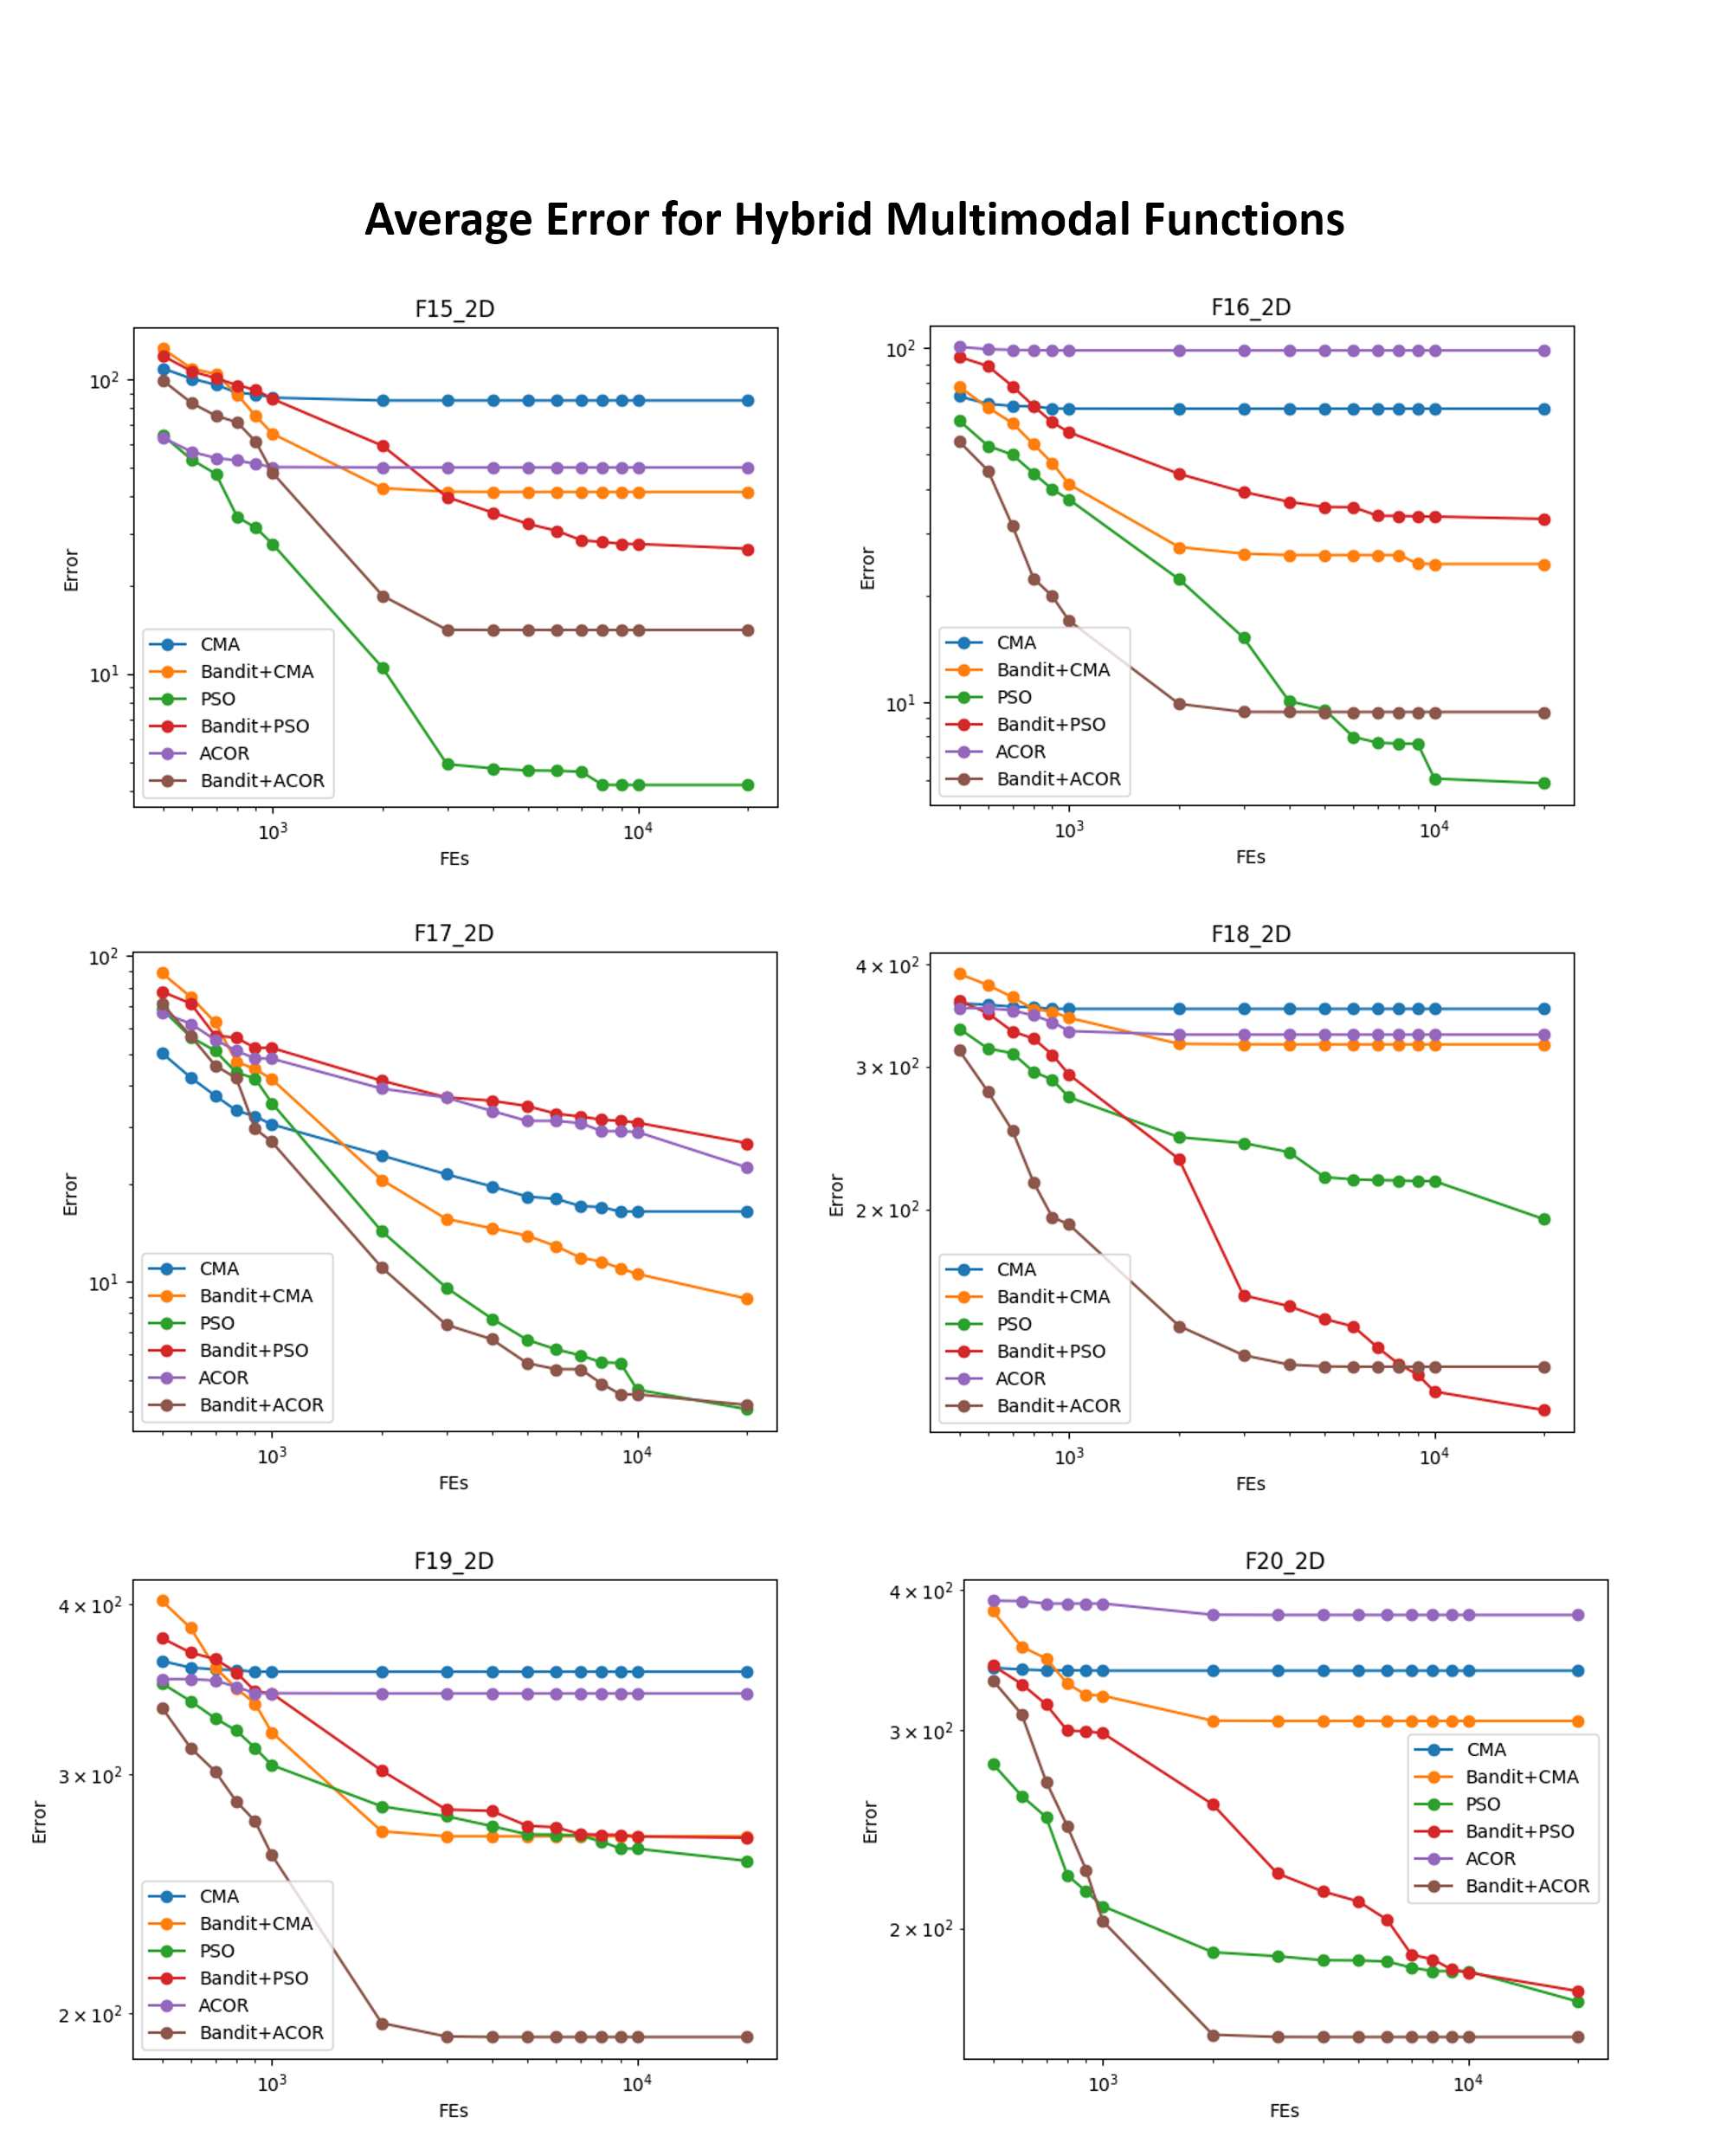
\includegraphics[width=\textwidth]{Average_F15_F20}
%\caption{Average Error for Hybrid Multimodal Functions.}\label{fig:Average_F15_F20}
%\end{figure} 
%
%\begin{figure}
%\centering
%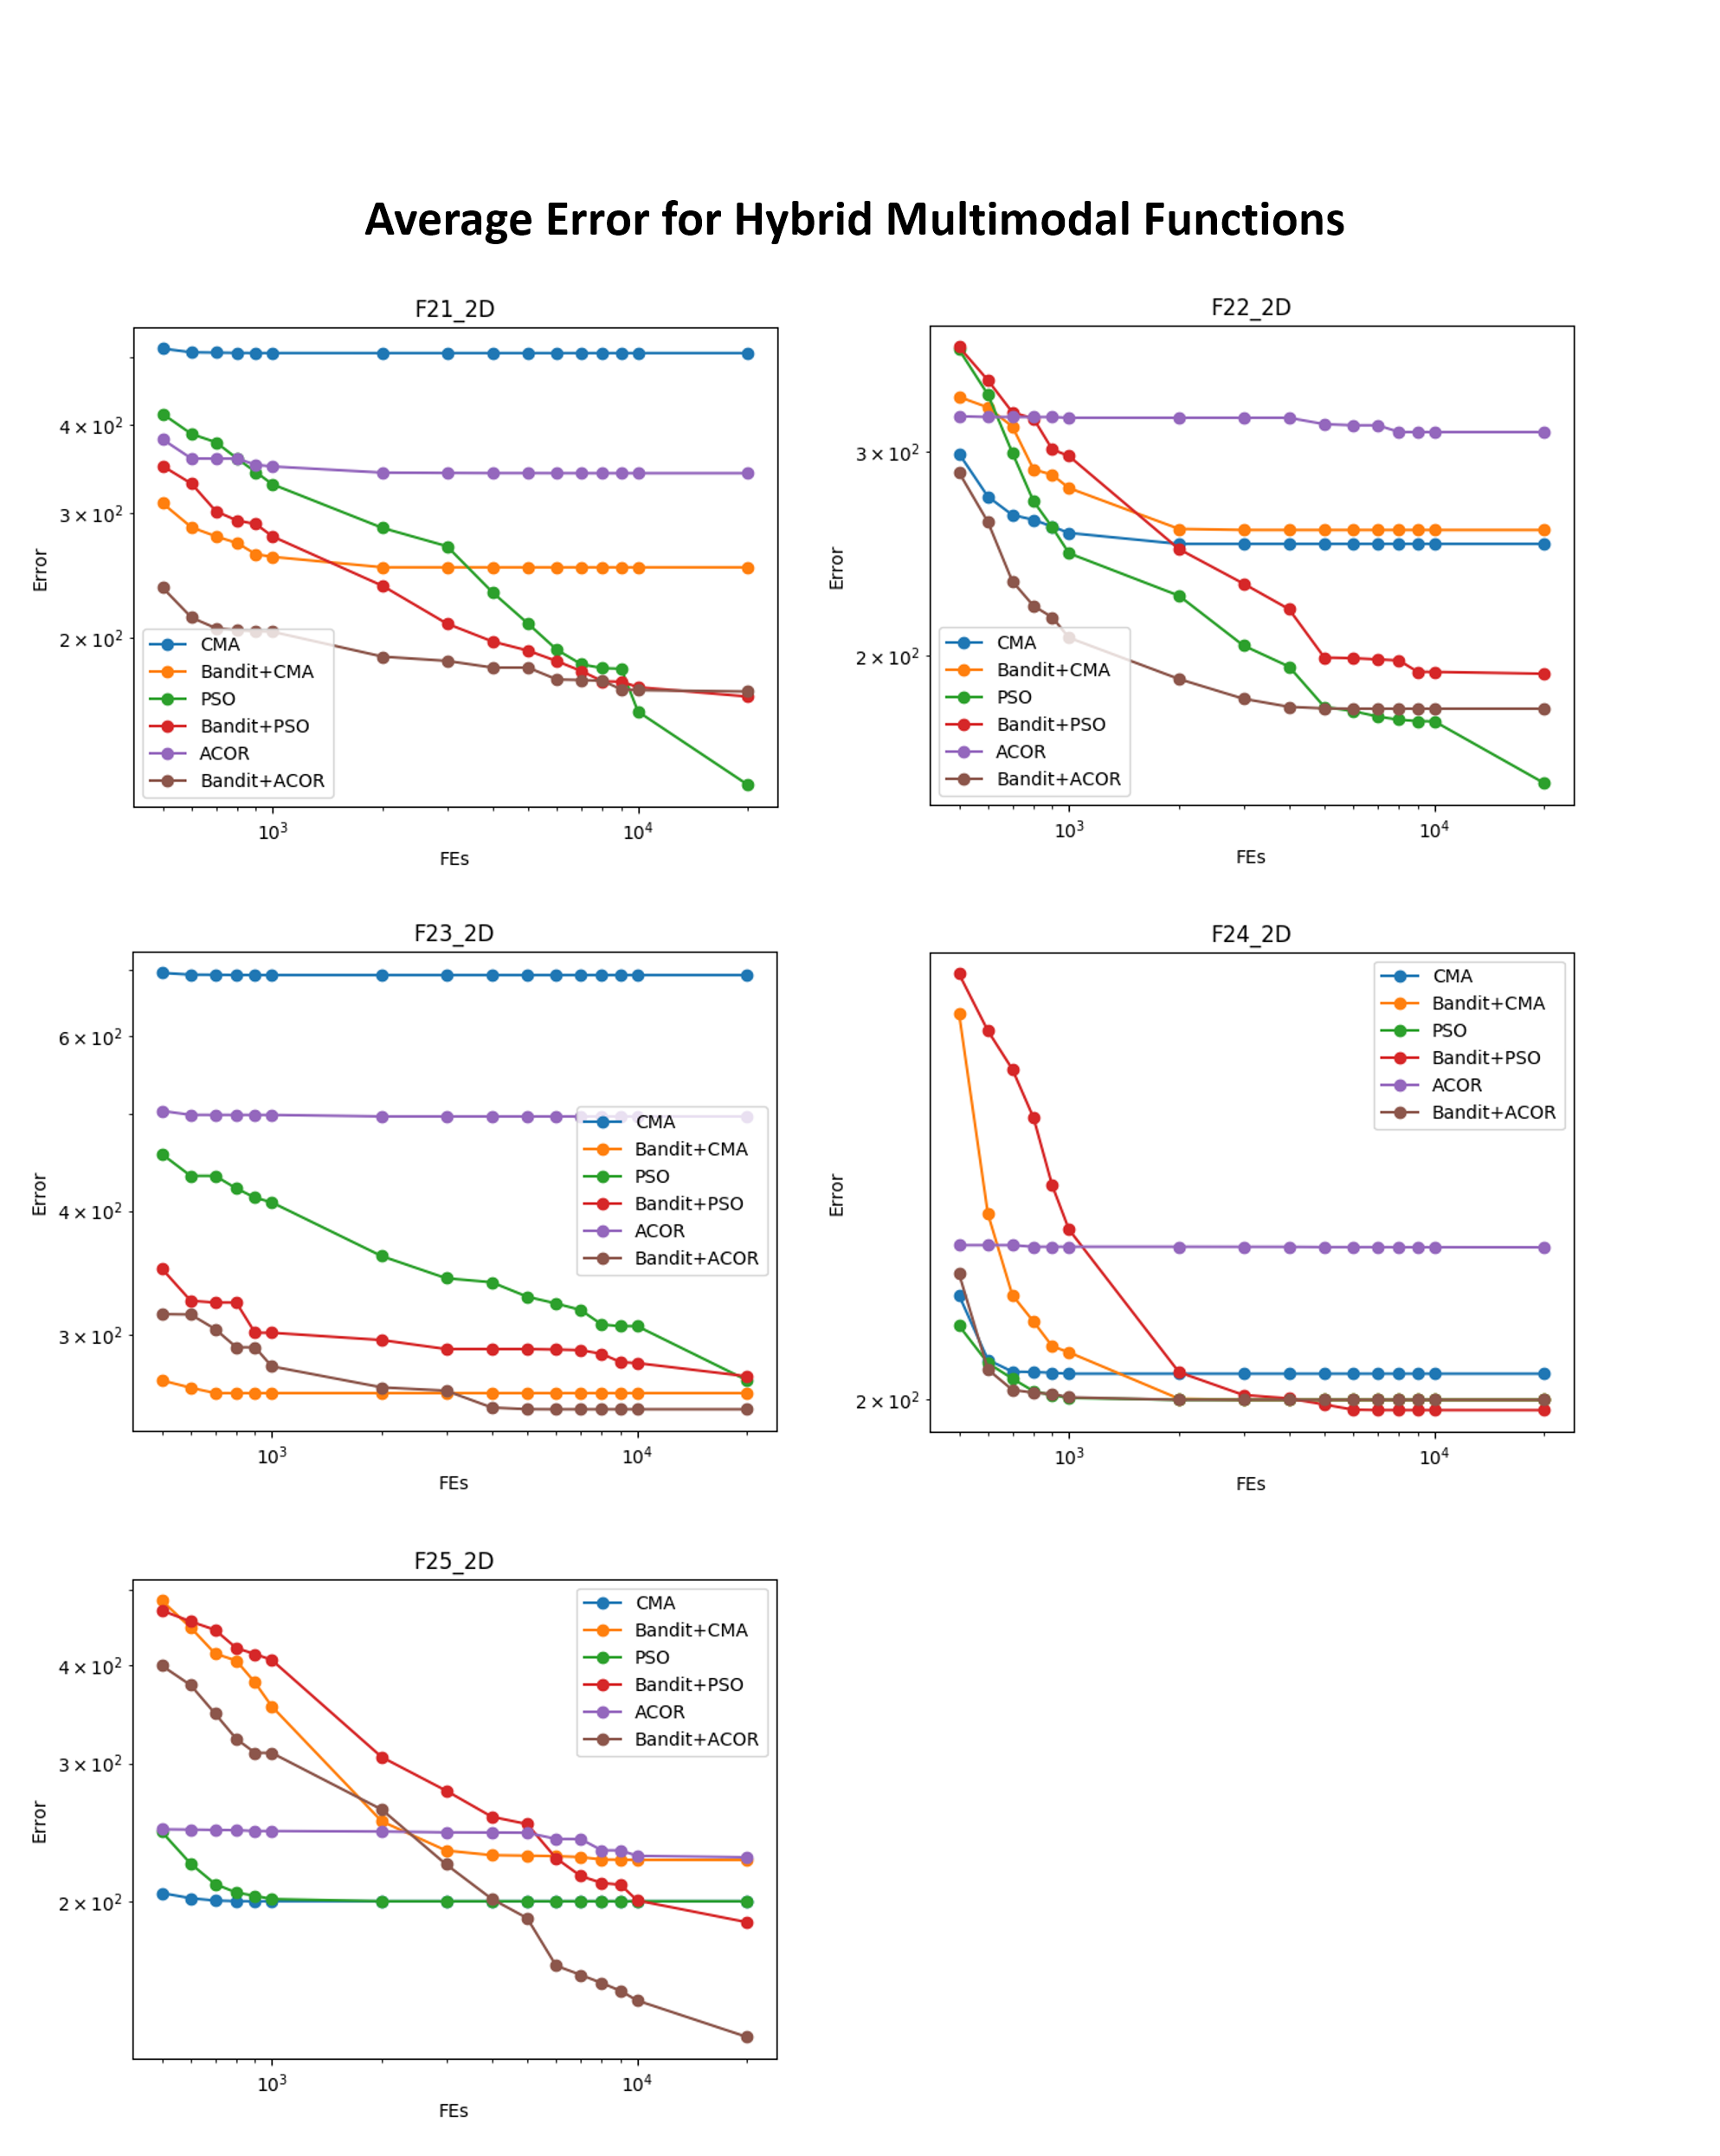
\includegraphics[width=\textwidth]{Average_F21_F25}
%\caption{Average Error for Hybrid Multimodal Functions.}\label{fig:Average_F21_F25}
%\end{figure} 
%
